\documentclass[10pt]{llncs}
\usepackage{amsmath, amssymb}
\setcounter{tocdepth}{3}
\usepackage{graphicx}
%\usepackage{psfig}
\usepackage{subfigure}
\usepackage{url}


%\usepackage{floatflt}
\urldef{\mailsa}\path|{alfred.hofmann, brigitte.apfel,
ursula.barth, christine.guenther,|
\urldef{\mailsb}\path|ingrid.haas, frank.holzwarth, anna.kramer,
leonie.kunz, nicole.sator,|
\urldef{\mailsc}\path|erika.siebert-cole, peter.strasser,
lncs}@springer.com|
\newcommand{\keywords}[1]{\par\addvspace\baselineskip
\noindent\keywordname\enspace\ignorespaces#1}

\begin{document}

\mainmatter  % start of an individual contribution

\title{Multiple Tracking with single Camera}

\titlerunning{}

\author{Giorgio Gemignani \inst{1} }
%
\authorrunning{G. Gemignani}

\institute{ DSA - University of Naples Parthenope \\ Centro
Direzionale, Isola C/4, 80143 Naples, Italy\\
%\email{giorgio.gemignani@uniparthenope.it}\\
}

\maketitle







%\begin{keywords}
%Video Surveillance, Stopped Object Detection, Neural Model, GPGPU.
%\end{keywords}
%\end{abstract}

\section{Abstract}
The theory of non-linear optimal filtering is formulated in terms of Bayesian inference and both the classical and recent filtering algorithms are derived using the same Bayesian notation and formalism.
Following the Bayesian perspective all algorithms are treated as approximations to certain probability distributions or their parameters describing both the uncertainties in the models and the physical randomness. 
The reason for choose the Bayesian philosophy makes easier to develop a consistent, practically applicable theory of recursive inference respect with for example, least squares or maximum likelihood approaches. 
Another useful consequence of selecting the Bayesian approach is that least squares, maximum likelihood and many other philosophically different results can be obtained as special cases or re-interpretations of the Bayesian results. 
Modeling uncertainty as randomness is a very “engineering” way of modeling
the world. It is exactly the approach also chosen in statistical physics as well as
in financial analysis. The Bayesian approach to optimal filtering is far from
new (see, e.g., Ho and Lee, 1964; Lee, 1964; Jazwinski, 1966; Stratonovich, 1968;
Jazwinski, 1970), because the theory already existed at the same time the seminal
article of Kalman (1960b) was published. The Kalman filter was derived from the
least squares point of view, but the non-linear filtering theory has been Bayesian
from the beginning (see, e.g., Jazwinski, 1970).
The Bayesian concept of modeling unknown parameters as random variables is just a convenient way of representing uncertainty under the same formalism that is used for representing randomness, not implying that one believes that there really
is something random in the parameters - it .
Also random or stochastic processes appearing in the mathematical models are
not necessarily really random in physical sense, but instead, the randomness is
just a mathematical trick for taking into account the uncertainty in a dynamic
phenomenon of the real world.


\newpage
\section{Introduction}
Optimal filtering refers to the methodology that can be used for estimating the
state of a time-varying system, which is indirectly observed through noisy measurements. The state of the system refers to the collection of dynamic variables
such as position, velocities and accelerations or orientation and rotational motion
parameters, which describe the physical state of the system. The noise in the measurements refers to a noise in the sense that the measurements are uncertain, that is,
even if we knew the true system state the measurements would not be deterministic
functions of the state, but would have certain distribution of possible values. The
time evolution of the state is modeled as a dynamic system, which is perturbed
by a certain process noise. This noise is used for modeling the uncertainties in
the system dynamics and in most cases the system is not truly stochastic, but the
stochasticity is only used for representing the model uncertainties.
Phenomena, which can be modeled as time varying systems of the above type are
very common in engineering applications. These kind of models can be found, for
example, in navigation, aerospace engineering, space engineering, remote surveillance, telecommunications, physics, audio signal processing, control engineering,
finance and several other fields. Examples of such applications are the following:

\begin{itemize}
\item  Global positioning system (GPS) 
(Kaplan, 1996) is a widely used satellite
navigation system, where the GPS receiver unit measures arrival times of
signals from several GPS satellites and computes its position based on these
measurements. The GPS receiver typically uses an extended Kalman filter
or some other optimal filtering algorithm for computing the position and
velocity such that the measurements and the assumed dynamics (laws of
physics) are taken into account. Also the ephemeris information, which is
the satellite reference information transmitted from the satellites to the GPS
receivers is typically generated using optimal filters.
\item Target tracking (Bar-Shalom et al., 2001; Crassidis and Junkins, 2004) refers
to the methodology, where a set of sensors such as active or passive radars,
radio frequency sensors, acoustic arrays, infrared sensors and other types
of sensors are used for determining the position and velocity of a remote
target. When this tracking is done continuously, the dynamics of the target
and measurements from the different sensors are most naturally combined
using an optimal filter. The target in this (single) target tracking case can be,
for example, a robot, a satellite, a car or an airplane.
\item Multiple target tracking (Bar-Shalom and Li, 1995; Blackman and Popoli,
1999; Stone et al., 1999; Särkkä et al., 2007b) systems are used for remote
surveillance in the cases, where there are multiple targets moving at the
same time in the same geographical area. This arises the concept of data
association (which measurement was from which target?) and the problem
of estimating the number of targets. Multiple target tracking systems are
typically used in remote surveillance for military purposes, but possible civil
applications are, for example, monitoring of car tunnels, automatic alarm
systems and people tracking in buildings.
Inertial navigation (Titterton and Weston, 1997; Grewal et al., 2001) uses
inertial sensors such as accelerometers and gyroscopes for computing the
position and velocity of a device such as a car, an airplane or a missile.
When the inaccuracies in sensor measurements are taken into account the
natural way of computing the estimates is by using an optimal filter. Also
in sensor calibration, which is typically done in time varying environment
optimal filters are often applied.
\item Integrated inertial navigation (Grewal et al., 2001; Bar-Shalom et al., 2001)
combines the good sides of unbiased but inaccurate sensors, such as altime-
ters and landmark trackers, and biased but locally accurate inertial sensors.
Combining of these different sources of information is most naturally per-
formed using an optimal filter such as the extended Kalman filter. This kind
of approach was used, for example, in the guidance system of Apollo 11
lunar module (Eagle), which landed on the moon in 1969.
\item GPS/INS navigation (Grewal et al., 2001; Bar-Shalom et al., 2001) is a form
of integrated inertial navigation, where the inertial sensors are combined
with a GPS receiver unit. In GPS/INS navigation system the short term
fluctuations of the GPS can be compensated with the inertial sensors and
the inertial sensor biases can be compensated with the GPS receiver. An
additional advantage of this approach is that it is possible to temporarily
switch to pure inertial navigation, when the GPS receiver is unable to com-
pute its position (i.e., has no fix) for some reason. This happens, for example,
indoors, in tunnels and in other cases when there is no direct line-of-sight
between the GPS receiver and the satellites.
\item Spread of infectious diseases (Anderson and May, 1991) can often be mod-
eled as differential equations for the number of susceptible, infected and re-
covered/dead individuals. When uncertainties are induced into the dynamic
equations, and when the measurements are not perfect, the estimation of the
spread of the disease can be formulated as an optimal filtering problem.
\item Biological processes (Murray, 1993) such as population growth, predator-
pray models and several other dynamic processes in biology can also be
modeled as (stochastic) differential equations. The estimation of the states
of these processes from inaccurate measurements can be formulated as an
optimal filtering problem.
\item Telecommunications is also a field where optimal filters are traditionally
used. For example, optimal receivers, signal detectors and phase locked
loops can be interpreted to contain optimal filters (Van Trees, 1968, 1971)
as components. Also the celebrated Viterbi algorithm (Viterbi, 1967) can be
interpreted as a combination of optimal filtering and optimal smoothing of
the underlying hidden Markov model.
\item Audio signal processing applications such as audio restoration (Godsill and
Rayner, 1998) and audio signal enhancement (Fong et al., 2002) often use
TVAR (time varying autoregressive) models as the underlying audio signal
models. These kind of models can be efficiently estimated using optimal
filters and smoothers.
\item Stochastic optimal control (Maybeck, 1982b; Stengel, 1994) considers con-
trol of time varying stochastic systems. Stochastic controllers can typically
be found in, for example, airplanes, cars and rockets. The optimality, in
addition to the statistical optimality, means that control signal is constructed
to minimize a performance cost, such as expected time to reach a predefined
state, the amount of fuel consumed or average distance from a desired po-
sition trajectory. Optimal filters are typically used for estimating the states
of the stochastic system and a deterministic optimal controller is constructed
independently from the filter such that it uses the estimate of the filter as
the known state. In theory, the optimal controller and optimal filter are not
completely decoupled and the problem of constructing optimal stochastic
controllers is far more challenging than constructing optimal filters and (de-
terministic) optimal controllers separately.
\item Learning systems or adaptive systems can often be mathematically formu-
tions has close relationship with Bayesian non-parametric modeling, ma-
chine learning and neural network modeling (MacKay, 1998; Bishop, 1995).
Methods, which are similar to the data association methods in multiple target
tracking are also applicable to on-line adaptive classification (Andrieu et al.,
2002). The connection between Gaussian process regression and optimal
filtering has also been recently discussed in Särkkä et al. (2007a) and Har-
tikainen and Särkkä (2010).
\item Physical systems which are time varying and measured through unideal sen-
sors can sometimes be formulated as stochastic state space models, and the
time evolution of the system can be estimated using optimal filters (Kaipio
and Somersalo, 2005). In Vauhkonen (1997) and more recently, for example,
in Pikkarainen (2005) optimal filtering is applied to Electrical Impedance
Tomography (EIT) problem in time varying setting and in Hiltunen et al.
(2011) to the Diffuse Optical Tomography (DOT).
\end{itemize}

\subsection{Origins of Bayesian Optimal Filtering} 

The roots of Bayesian analysis of time dependent behavior are in the optimal linear
filtering. The idea of constructing mathematically optimal recursive estimators was
first presented for linear systems due to their mathematical simplicity and the most natural optimality criterion in both mathematical and modeling point of view was the least squares optimality. For linear systems the optimal Bayesian solution (with MMSE utility) coincides with the least squares solution, that is, the optimal least squares solution is exactly the posterior mean.\\
The history of optimal filtering starts from the Wiener filter (Wiener, 1950), which is a spectral domain solution to the problem of least squares optimal filtering of stationary Gaussian signals. The Wiener filter is still important in communication applications (Proakis, 2001), digital signal processing (Hayes, 1996) and image processing (Rafael C. Gonzalez, 2008). The disadvantages of the Wiener filter are that it can only be applied to stationary signals and that the construction of a Wiener filter is often mathematically demanding and these mathematics cannot be avoided (i.e., made transparent).\\
Due to the demanding mathematics the Wiener filter can only be applied to simple low dimensional filtering problems. The success of optimal linear filtering in engineering applications is mostly due to the seminal article of Kalman (1960b), which describes the recursive solution to the optimal discrete-time (sampled) linear filtering problem. The reason to the success is that the Kalman filter can be understood and applied with very much lighter mathematical machinery than the Wiener filter. \\
Also, despite its mathematical simplicity, the Kalman filter (or actually the Kalman-Bucy filter; Kalman and Bucy, 1961) contains the Wiener filter as its limiting special case.In the early stages of its history, the Kalman filter was soon discovered to belong to the class of Bayesian estimators (Ho and Lee, 1964; Lee, 1964; Jazwinski, 1966, 1970). \\
An interesting historical detail is that while Kalman and Bucy were formulating the linear theory in the United States, Stratonovich was doing the pioneering work on the probabilistic (Bayesian) approach in Russia (Stratonovich, 1968; Jazwinski, 1970).
As discussed in the book of West and Harrison (1997), in the sixties, Kalman filter like recursive estimators were also used in the Bayesian community and it is not clear whether the theory of Kalman filtering or the theory of dynamic linear models (DLM) was the first. Although these theories were originally derived from slightly different starting points, they are equivalent. Because of Kalman filter’s useful connection to the theory and history of stochastic optimal control, this document approaches the Bayesian filtering problem from the Kalman filtering point of view.\\
Although the original derivation of the Kalman filter was based on the least squares approach, the same equations can be derived from the pure probabilistic Bayesian analysis. The Bayesian analysis of Kalman filtering is well covered in the classical book of Jazwinski (1970) and more recently in the book of Bar-Shalom et al. (2001). Kalman filtering, mostly because of its least squares interpretation, has widely been used in stochastic optimal control. \\
A practical reason to this is that the inventor of the Kalman filter, Rudolph E. Kalman, has also made several contributions (Kalman, 1960a) to the theory of linear quadratic Gaussian (LQG) regulators, which are fundamental tools of stochastic optimal control (Stengel,1994; Maybeck, 1982b).\\ 
Optimal Bayesian filtering (see, e.g. Jazwinski, 1970; Bar-Shalom et al., 2001;Doucet et al., 2001; Ristic et al., 2004) considers statistical inversion problems, where the unknown quantity is a vector valued time series $(x_1 , x_2 , . . x_T)$ which is observed through noisy measurements $(y_1 , y_2 , . . ,y_T)$ as illustrated in the Figure 1.4.
An example of this kind of time series is shown in the Figure 1.5. 
The process shown is actually a discrete-time noisy resonator with a known angular velocity.The state $ x_k = ( x_{k}  x_k )^T $ is two dimensional and consists of the position of the resonator $x_k$ and its time derivative $x_k$ . The measurements $y_k$ are scalar observations of the resonator position (signal) and they are corrupted by measurement noise.
The purpose of the statistical inversion is to estimate the hidden states 
$X=(x_1 , . . . , x_T)$ given the observed measurements $Y=(y_1 , . . . , y_T)$, which means that in the Bayesian sense (Bernardo and Smith, 1994; Gelman et al., 1995) equals to compute the joint posterior distribution of all the states given all the measurements.\\\
This can be done by straightforward application of the Bayes rule:

\begin{equation}  \label{eqn: Bayes rule}
p(x_1 , x_2 , . . x_T | y_1 , y_2 , . . ,y_T)=
\frac{ p(y_1 , . . ,y_T | x_1 , . ., x_T  ) p(x_1 , . . ,x_T) }{p(y_1,..,y_T)}
\end{equation}

where:

\begin{itemize}
\item $p(x_1,...,x_T)$ is \textit{the prior} defined by the dinamical model,

\item $p(y_1 , . . ,y_T | x_1 , . ., x_T)$ is the \textit{likelihood} model for the measurements,

\item $p(y_1,..,y_T)$ is the \textit{evidence} factor defined as: 

\begin{eqnarray} \label{eqn: Evidence eq}
p(y_1,..,y_T)=
\int p(y_1 , . . ,y_T , x_1 , . ., x_T  ) d(x_1 , . ., x_T ) \nonumber \\
\int p(y_1 , . . ,y_T | x_1 , . ., x_T  ) p(x_1 , . ., x_T ) d(x_1 , . ., x_T )
\end{eqnarray}

\end{itemize}
Unfortunately, this full posterior formulation has the serious disadvantage that each
time we obtain a new measurement, the full posterior distribution would have to
be recomputed. \\
This is particularly a problem in dynamic estimation (which is exactly the problem we are solving here!), because there measurements are typically obtained one at a time and we would want to compute the best possible estimate after each measurement. When number of time steps increases, the dimensionality of the full posterior distribution also increases, which means that the computational complexity of a single time step increases.\\
Thus after a sufficient number of time steps the computations will become intractable, independently of available computational resources. Without additional information or harsh approximations, there is no way of getting over this problem in the full posterior computation.\\
However, the above problem only arises when we want to compute the full posterior distribution of the states at each time step. If we are willing to relax this a bit and be satisfied with selected marginal distributions of the states, the computations become order of magnitude lighter. In order to achieve this, we also need to restrict the class of dynamic models into probabilistic Markov sequences, which as a restriction sounds more restrictive than it really is.\\
The model for the states and measurements will be assumed to be of the following type:\\
\begin{itemize}

\item \textbf{Initial distribution} specifies \textit{the prior distribution} $p(x_0 )$ of the hidden state $x_0$ at initial time step $k = 0$ ,

\item \textbf{Dynamic model} models the \textit{system dynamics and its uncertainties as a Markov sequence} , defined in terms of the transition distribution $p(x_k | x_{k−1} )$ ,

\item \textbf{Measurement model} models \textit{the relation} between the observed measurement $y_k$ on the current state $x_k$ . This dependence is modeled by specifying the distribution of the measurement given the state $p(y_k | x_k )$ .
\end{itemize}

Because computing the full joint distribution of the states at all time steps is computationally very inefficient and unnecessary in real-time applications, in optimal
(Bayesian) filtering the following marginal distributions are considered instead:
\begin{itemize}
\item \textbf{Filtering distributions} are the marginal distributions of the current state $x_k$ given the previous measurements ${y_1 , . . . , y_k}$:

\begin{eqnarray} \label{eqn: Filtering distributions}
p(x_k | y_1 , . . . , y_k ), & k = 1, . . . , T.
\end{eqnarray}

\item \textbf{Prediction distributions} are the marginal distributions of the future states, $n$ steps after the current time step:
\begin{eqnarray} \label{eqn: Prediction distributions}
p(x_{k+n} | y_1 , . . . , y_k ) , k = 1, . . . , T , & n = 1, 2, . . . ,
\end{eqnarray}

\item \textbf{Smoothing distributions} are the marginal distributions of the states $x_k$ given a certain interval ${y_1 , . . . , y_T }$ of measurements with $T > k$:

\begin{eqnarray}\label{eqn: Smoothing distributions}
p(x_k | y_1 , . . . , y_T ), k = 1, . . . , T.
\end{eqnarray}

\end{itemize}


\subsection{Algorithms for Optimal Filtering and Smoothing}
There exists a few classes of filtering and smoothing problems which have closed
form solutions:
\begin{itemize}
\item \textit{Kalman filter} (\textbf{KF}) is a closed form solution to the discrete linear filtering problem. Due to linear Gaussian model assumptions the posterior distribution is exactly Gaussian and no numerical approximations are needed.
\item \textit{Rauch-Tung-Striebel smoother} (\textbf{RTSS}) is the corresponding closed form smoother
to linear Gaussian state space models.
\item \textit{Grid filters and smoothers}, are solutions to Markov models with finite state
spaces.But because the Bayesian optimal filtering and smoothing equations are generally
computationally intractable, many kinds of numerical approximation methods have
been developed, for example:
\item \textit{Extended Kalman filter} (\textbf{EKF}) approximates the non-linear and non-Gaussian
measurement and dynamic models by linearization, that is, by forming a
Taylor series expansion on the nominal (or Maximum a Posteriori, MAP)
solution. This results in Gaussian approximation to the filtering distribution.
\item \textit{Extended Rauch-Tung-Striebel} smoother (\textbf{ERTSS}) is the approximate non-
linear smoothing algorithm corresponding to EKF.
\item \textit{Unscented Kalman filter} (\textbf{UKF}) approximates the propagation of densities through the non-linearities of measurement and noise processes by unscented
transform. This also results in Gaussian approximation.
Unscented Rauch-Tung-Striebel smoother (\textbf{URTSS}) is the approximate non-
linear smoothing algorithm corresponding to UKF.
\item \textit{Sequential Monte Carlo methods or particle filters and smoothers} represent
the posterior distribution a as weighted set of Monte Carlo samples.
\item \textit{ Unscented particle filter} (\textbf{UPF}) and local linearization based methods use
\textbf{UKFs} and \textbf{EKFs}, respectively, for approximating the importance distribu-
tions in sequential importance sampling.
\item \textit{ Rao-Blackwellized particle filters and smoothers} use closed form integration (e.g., Kalman filters and \textbf{RTS} smoothers) for some of the state variables and Monte Carlo integration for others.
\item \textit{Interacting multiple models} (\textbf{IMM}), and other multiple model methods approximate the posterior distributions with mixture Gaussian approximations.
\item \textit{Grid based methods} approximate the distribution as a discrete distribution
defined in a finite grid.
\item Other methods also exists, for example, based on series expansions, describ-
ing functions, basis function expansions, exponential family of distributions,
variational Bayesian methods, batch Monte Carlo (e.g., MCMC), Galerkin
approximations etc.
\end{itemize}




\newpage



\chapter*{Probabilistic Bayesian Filtering}
\section{Introduction}
In this chapter the theory of probabilistic Bayesian filtering (PBF) is presented. The Kalman filtering equations, which are the closed form solutions to the linear Gaussian discrete-time optimal filtering problem, are also derived.

\section{Probabilistic Filtering Equations and Exact Solutions}
Before going into the practical non-linear filtering algorithms, we first present the classical formulation of the discrete-time optimal filtering as recursive Bayesian inference. Then the classical Kalman filters, extended Kalman filters and statistical linearization based filters are presented in terms of the general theory. 
\newtheorem {thm}{Definition}[section]

\begin{thm}[State space model]. 
Discrete-time state space model or probabilistic non-linear filtering model is a recursively defined probabilistic model of the form

\begin{eqnarray} \label{eqn: State space model}
x_k & \approx & p(x_k | x_{k-1} ) \nonumber \\
y_k &  \approx & p(y_k | x_k ) 
\end{eqnarray}

where:

\begin{itemize}
\item $x_k \in \Re_{n}$ is the state of the system on the time step $k$.
\item $y_k \in \Re_{n}$ is the measurement on the time step $k$.
\item $p(x_k | x_{k-1})$ is the dynamic model, which models the stochastic dynamics of the system. The dynamic model can be a probability density, a counting measure or combination of them depending on if the state $x_k$ is continuous, discrete or hybrid.
\item $p(y_k | x_k )$ is the measurement model, which models the distribution of the
measurements given the state.
\end{itemize}

\end{thm}

The model is assumed to be Markovian, which means that it has the following two properties:
\newtheorem{thm1}{Property}[section]

\begin{thm1} [Markov property of states]
States $\{x_k : k = 1, 2, . . .\}$ form a Markov sequence (or Markov chain if the state
is discrete). This Markov property means that $x_k$ (and actually the whole future
$(x_{k+1} , x_{k+2} , . . .)$ given $x_{k-1}$ is independent from anything that has happened in the past:

\begin{eqnarray} \label{eqn: Indipendence State1}
p(x_k | x_{1:k−1} , y_{1:k−1} ) = p(x_k | x_{k-1} ).
\end{eqnarray}

Also the past is independent of the future given the present:
\begin{eqnarray} \label{eqn: Indipendence State2}
p(x_{k-1} | x_{k:T} , y_{k:T} ) = p(x_{k-1} | x_k ).
\end{eqnarray}
\end{thm1} 

\newtheorem{thm2}{Property}[section]

\begin{thm2} [Conditional independence of mesaurements]
The measurement $y_k$ given the state $x_k$ is conditionally independent from the mea-
surement and state histories:
 \begin{eqnarray} \label{eqn: Indipendence Measurement}
 p(y_{k} | x_{1:k} , y_{1:k-1} ) = p(y_k | x_k ).
 \end{eqnarray}
\end{thm2}

The filtering model can be equivalently expressed as an Hidden Markov chain or a directed  graphical model whose representation is depicted in figure \ref{fig:GM}
\begin{figure}[!htb]\label{fig:GM}
\begin{center}
 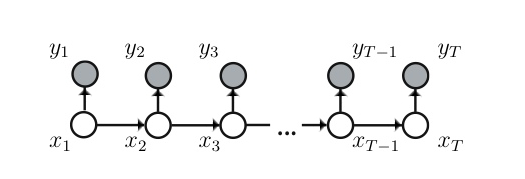
\includegraphics[width=10cm]{./ImaginiLatex/gm_directed.eps} 
\end{center}
\caption{The directed graph of the Filtering Model. The link  $x_k$ and $x_{k-1}$ express the markov property while the link between $y_k$ and $x_k$ express the conditional indipendence property of measurements}

\end{figure}

Following the factorization theorem for the directed graphical models:
\begin{eqnarray} \label{eqn: Full Joint Distribution}
p(x_0 , . . . , x_T,y_1 , . . . , y_T ) = p(x_0 ) \prod_{k=1}^{T} p(x_k | x_{k-1} ) = \nonumber \\
\prod_{k=1}^{T} p(y_k | x_{k} ) 
\end{eqnarray}

Marginalizing out $Y=\{y_1 , . . . , y_T\}$ from the joint distribution we obtain
the joint prior distribution of the states $X={x_0 , . . . , x_T}$ :
\begin{eqnarray} \label{eqn: joint states distribution}
p(x_0 , . . . , x_T ) = \int p(y_1 , . . ,y_T , x_1 , . ., x_T) d(y_1 , . ., y_T) =  \nonumber \\
p(x_0 ) \prod_{k=1}^{T} p(x_k | x_{k - 1} ) 
\end{eqnarray}

Applying the bayes rule to \ref{eqn: Full Joint Distribution} and \ref{eqn: joint states distribution} we can compute the joint likelihood of measurements $Y=\{y_1 , . . . , y_T\}$:
\begin{eqnarray} \label{eqn: joint measurements likelyhood}
p(y_1 , . . . , y_T | x_0 , . . . , x_T ) = \nonumber \\
\frac{p(y_1 , . . ,y_T,x_1 , . ., x_T)}{ p(x_0,x_1 , . ., x_T)} = \nonumber \\
\prod_{k=1}^{T} p(y_k | x_k) 
\end{eqnarray}

In principle, for given $T$ we could simply compute the posterior distribution of the
states by the Bayes rule:

\begin{eqnarray}  \label{eqn: Bayes rule2}
p(x_0,x_1 , x_2 , . . x_T | y_1 , y_2 , . . ,y_T)= 
\frac{ p(y_1 , . . ,y_T | x_1 , . ., x_T )p(x_1 , . . ,x_T) } {p(y_1,..,y_T)} \nonumber \\
\approx p(y_1 , . . ,y_T | x_1 , . ., x_T  ) p(x_1 , . . ,x_T)
\end{eqnarray}

However, this kind of explicit usage of the full Bayes’ rule is not feasible in real
time applications, because the amount of computations per time step increases
when new observations arrive. Thus, this way we could only work with small data
sets, because if the amount of data is not bounded (as in real time sensoring appli-
cations), then at some point of time the computations would become intractable.
To cope with real time data we need to have an algorithm which does constant
amount of computations per time step.
As discussed in Section 1.2.3, filtering distributions, prediction distributions
and smoothing distributions can be computed recursively such that only constant
amount of computations is done on each time step. For this reason we shall not con-
sider the full posterior computation at all, but concentrate to the above-mentioned
distributions instead.

\section{Optimal Filtering Equations}
The purpose of optimal filtering is to compute the marginal posterior distribution
of the state $x_k$ on the time step $k$ given the history of the measurements up to the
time step $k$
\begin{eqnarray} \label{eqn: Optimal Filtering Equations}
p(x_k | y_{1:k} ). 
\end{eqnarray} 

The fundamental equations of the Bayesian filtering theory are given by the fol-
lowing theorem:
\newtheorem{thm3}{Theorem}[section]

\begin{thm3} [Bayesian optimal filtering equations]
The recursive equations for computing the predicted distribution $p(x_k | y_{1:k-1})$ and the filtering distribution $p(x_k | y_{1:k})$ on the time step $k$ are given by the following Bayesian filtering steps:
\begin{enumerate}
\item \textbf{Initialization}. The recursion starts from the prior distribution $p(x_0 )$.
\item \textbf{Prediction}. The predictive distribution of the state $x_k$ on time step $k$ given the dynamic model can be computed by the \textbf{Chapman-Kolmogorov} equation

\begin{eqnarray} \label{eqn: Prediction Step}
p(x_k | y_{1:k-1} ) =p(x_k | x_{k-1} ) p(x_{k-1} | y_{1:k-1} ) dx_{k-1} .
\end{eqnarray}

\item \textbf{Update}. Given the measurement $y_k$ on time step $k$ the posterior distribution of the state $xk$ can be computed by the Bayes’ rule
\begin{eqnarray} \label{eqn: Update Step}
p(x_k | y_{1:k} ) = \frac{1}{Z_k} p(y_k | x_k ) p(x_k | y_{1:k-1} ),
\end{eqnarray}

where the normalization constant $Z_k$ is given as
\begin{eqnarray} \label{eqn: Normalization}
Z_k = p(y_k | x_k ) p(x_k | y_{1:k-1} ) dx_k .
\end{eqnarray}
\end{enumerate}

If some of the components of the state are discrete, the corresponding integrals are
replaced with summations.
\end{thm3}

\textit{Proof.} The joint distribution of $x_k$ and $x_{k-1}$ given $y_{1:k-1}$ can be computed as
\begin{eqnarray} \label{eqn: prof1}
p(x_k , x_{k-1} | y_{1:k-1} ) =   \frac{p(x_k , x_{k-1} , y_{1:k-1})}{p(y_{1:k-1})} = \nonumber \\
\frac{p(x_k | x_{k-1} , y_{1:k-1}) p(x_{k-1} , y_{1:k-1}) }{p(y_{1:k-1})} =
 p(x_k | x_{k-1} , y_{1:k-1}) p(x_{k-1} | y_{1:k-1}) 
\end{eqnarray}

that can be further simplified by the Independence properties of Markov assumption \ref{eqn: Indipendence State1} and \ref{eqn: Indipendence State2} in 
\begin{eqnarray} \label{eqn: prof2}
p(x_k , x_{k-1} | y_{1:k-1} )= p(x_k | x_{k-1} ) p(x_{k-1} | y_{1:k-1} )
\end{eqnarray}


The marginal distribution of $x_k$ given $y_{1:k-1}$ can be obtained marginalizing out the  $x_{k-1}$ from the distribution
\footnote{This arise applying the simple substitution to the joint distribution of 3 events
$A$,$B$ and $C$:
$$
p(A|C)=\int \frac{p(A,B,C)}{p(C)}dB=\frac{1}{p(C)}\int p(A,B,C)dB =\frac{p(A,C)}{p(C)}
$$
} 
 \label{eqn: prof2} giving the Chapman-Kolmogorov equation

\begin{eqnarray} \label{eqn: Chapman-Kolmogorov}
p(x_k | y_{1:k-1} )= \int p(x_k | x_{k-1} ) p(x_{k-1} | y_{1:k-1} ) dx_{k-1}
\end{eqnarray}

If $x_{k-1}$ is discrete, then the above integral is replaced with sum over $x_{k-1}$ .
The normalization factor $Z_k$ in can be expressed as:
\begin{eqnarray} \label{eqn: Normalization1}
Z_k =  p(y_k | y_{1:k-1})= \frac{p(y_k , y_{1:k-1})}{p( y_{1:k-1})} = 
\int \frac{ p( y_k , y_{1:k-1} , x_k) }{ p( y_{1:k-1}) } dx_k =  \\
\int \frac{ p(y_k | x_k , y_{1:k-1}) p(x_k , y_{1:k-1}) }{ p( y_{1:k-1}) } dx_k = 
\int \frac{ p(y_k | x_k) p(x_k , y_{1:k-1}) }{ p( y_{1:k-1}) } dx_k = \\
=\int p(y_k | x_k ) p(x_k | y_{1:k-1} ) dx_k
\end{eqnarray}

The posterior distribution of $x_k$ given $y_k$ and $y_{1:k-1}$ can be computed as:
\begin{eqnarray} \label{eqn: Posterior}
p(x_k | y_{1:k} )=  \frac{ p(x_k , y_k , y_{1:k-1} )}{ p(y_k , y_{1:k-1})} =
 \frac{ p(y_k | x_k , y_{1:k-1}) p(x_k , y_{1:k-1}) }{  p(y_k , y_{1:k-1})} = \\
 \frac{ p(y_k | x_k) p(x_k , y_{1:k-1}) }{ p(y_k , y_{1:k-1}) } =
 \frac{ p(y_k | x_k) p(x_k | y_{1:k-1}) p(y_{1:k-1}) }{ p(y_k , y_{1:k-1}) } = \\
 \frac{ p(y_k | x_k) p(x_k | y_{1:k-1})}{ p(y_k | y_{1:k-1}) } =
 \frac{1}{Z_k} p(y_k | x_k) p(x_k | y_{1:k-1})
\end{eqnarray}

 
\chapter*{Markov Chain Monte Carlo}
\section{Introduction}
The application of probabilistic models to data often leads to inference problems that require the integration of complex, high dimensional distributions. Markov chain Monte Carlo (\textbf{MCMC}), is a general computational approach that replaces analytic integration by summation over samples generated from iterative algorithms.\\
Problems that are intractable using analytic approaches often become possible to solve using some form of \textbf{MCMC}, even with high-dimensional problems. \\
The development of \textbf{MCMC} is arguably the biggest advance in the computational approach to statistics. While \textbf{MCMC} is very much an active research area, there are now some standardized techniques that are widely used. In this chapter, after a brief introduction on the two main key ingredients of \textbf{MCMC} which are Monte Carlo integration and Markov chains, will discuss two forms of \textbf{MCMC}: \textit{Metropolis-Hastings} and \textit{Gibbs sampling}. 
\section{Monte Carlo Integration}
Many problems in probabilistic inference require the calculation of complex integrals or
summations over very large outcome spaces. For example, a frequent problem is to calculate
$E[g(x)]$,the expectation of a function $g(x)$ for the random variable $x$ (for simplicity, we assume $x$ is a univariate random variable) definde
If $x$ is continuous, the expectation is defined as:
\begin{eqnarray} \label{eqn: Expectation}
E[g(x)] = \left\{
\begin{array}{ccccc}
\int g(x)p(x)dx  & \mbox{if} & $x$ & is & continuous \\
\sum g(x)p(x)dx  & \mbox{if} & $x$ & is & discrete
\end{array}
\right.
\end{eqnarray}

These expectations arise in many situations where we want to calculate some statistic of a
distribution, such as the mean or variance. For example, if $g(x) = x$, we are calculating the mean of a distribution. Integration or summation using analytic techniques can become
quite challenging for certain distributions. For example, the density $p(x)$ might have a
functional form that does not lend itself to analytic integration. For discrete distributions, the outcome space might become so large to make the explicit summation over all possible outcomes impractical.\\
The general idea of Monte Carlo integration is to use samples to approximate the expectation of a complex distribution. Specifically, we obtain a set of samples $x(i), i = 1, . . . , N,$ drawn independently from distribution $p(x)$. In this case, we can approximate the expectations in \ref{eqn: Expectation} by a finite sum:
\begin{eqnarray} \label{eqn: Expectation Approx}
E[g(x)] = \sum_{i=1}^N g(x^i)p(x^i)
\end{eqnarray}
In this procedure, we have now replaced analytic integration with summation over a
suitably large set of samples. Generally, the accuracy of the approximation can be made as
accurate as needed by increasing $n$. Crucially, the precision of the approximation depends
on the independence of the samples: when the samples are correlated, the effective sample
size decreases.

\section{Markov Chain}
A Markov chain is a stochastic process where we transition from one state to another state
using a simple sequential procedure. We start a Markov chain at some state $x^1$, and use
a \textit{transition function} $p(x^t|x^{t-1})$, to determine the next state, $x^2$ conditioned on the last observed state. 
We then keep iterating to create a sequence of states:
$$
x^1  \rightarrow  x^2  \rightarrow . . . → x^t  \rightarrow . . .
$$
Each such a sequence of states is called a Markov chain or simply chain. The procedure
for generating a sequence of $T$ states from a Markov chain is the following:\\
{\bf MARKOV CHAIN GENERATION}\\[.4cm]
{\sf
0. \hspace*{0.2cm} Set $t=1$  \\
1. \hspace*{0.2cm} Generate a initial value $u$, and $set x^t = u$\\
3. \hspace*{0.2cm}  Repeat\\
3.1 \hspace*{0.3cm} $t=t+1$\\
3.2 \hspace*{0.3cm} Sample a new value $u$ from the transition function $p( x^t |x^{t-1})$\\
3.3 \hspace*{0.3cm} Set $x^t = u$\\
4. Until $t = T$\\
}\\[.4cm]
\\
\\


Importantly, in this iterative procedure, the next state of the chain at $t+1$ is based only on the previous state at t. Therefore, each Markov chain wanders around the state space and the transition to a new state is only dependent on the last state, giving to the whole procedure a \"memoryless\" property.
This local dependency behavior is an important property when using Markov chains for MCMC.
When initializing each Markov chain, the chain will wander in state space around the
starting state. Therefore, if we start a number of chains, each with different initial conditions, the chains will initially be in a state close to the starting state. This period is called the \textit{burnin}. An important property of Markov chains is that the starting state of the chain nolonger affects the state of the chain after a sufficiently long sequence of transitions (assuming that certain conditions about the Markov chain are met). At this point, the chain is said to reach its \textit{steady state} and the states reflect samples from its stationary distribution.
\\ This property that Markov chains converge to a stationary distribution regardless of where we started (if certain regularity conditions of the transition function are met), is quite important.
When applied to MCMC, it allow us to draw samples from a distribution using a sequential
procedure but where the starting state of the sequence does not affect the estimation process.
\newpage
\section{Markov chain Monte Carlo}
The two previous sections discussed the main two ideas underlying MCMC, Monte Carlo
sampling and Markov chains. Monte Carlo sampling allows one to estimate various characteristics of a distribution such as the mean, variance, kurtosis, or any other statistic of interest to a researcher. Markov chains involve a stochastic sequential process where we can sample states from some stationary distribution.\\
The goal of MCMC is to design a Markov chain such that the stationary distribution of
the chain is exactly the distribution that we are interesting in sampling from. This is called the \textit{target distribution}.\\
The target distribution could be the posterior distribution over the parameters in the model or the posterior predictive distribution of a model or any other distribution of interest to the researcher.\\
In other words, we would like the states sampled from some Markov chain to also be samples drawn from the target distribution. The idea is to use some clever methods for setting up the transition function such that no matter how we initialize each chain, we will convergence to the target distribution.\\
In the next section is discussed a general MCMC procedure and its modified version: Metropolis-Hastings and Metropolis.
\subsection{Metropolis sampler}
The Metropolis sampler is special case of the Metropolis-Hastings sampler discussed in the next section. Suppose our goal is to sample from the target density $p(\theta)$, with $-\inf < \theta < \inf$ . The Metropolis sampler creates a Markov chain that produces a sequence of states:
$$
\theta^1 \rightarrow  \theta^2 \rightarrow. . .  \rightarrow \theta^t  \rightarrow . . .
$$
where $\theta^t$ represents the state of a Markov chain at iteration $t$. 
The samples from the chain, after burnin, reflect samples from the target distribution $p(θ)$.\\
In the Metropolis procedure, we initialize the first state, $\theta^1$ to some initial value. We then use a proposal distribution $q(\theta^t|\theta^{t-1})$ to generate a candidate point $\theta^∗$ corresponding to a possible value for state at time $t$ conditioned on the previous state of the sampler. \\
The next step is to either accept the proposal or reject it. The probability $\alpha$ of accepting the proposal is definded as:\\
\begin{eqnarray} \label{eqn: Acceptance Ratio Metropolis}
\alpha = min(1, \frac{p(\theta^*)}{p(\theta^{t-1})})
\end{eqnarray}
To make a decision on whether to actually accept or reject the proposal, we generate a
uniform deviate $u$. If $u > \alpha$ , we accept the proposal and the next state is set equal to the proposal:  $\theta^t=\theta^{∗}$ . \\
 If $u \leq \alpha$, we reject the proposal, and the next state is set equal to the
old state: $\theta^t=\theta^{t-1}$ . We continue generating new proposals conditional on the current state of the sampler, and either accept or reject the proposals. This procedure continues until the sampler reaches convergence. At this point, the samples $\theta^t$ reflect samples from the target distribution $p(\theta)$. The Metropolis sampler algorithm is :\\
{\bf METROPOLIS Sampler}\\[.4cm]
{\sf
0. \hspace*{0.2cm} Set $t=1$  \\
1. \hspace*{0.2cm} Generate a initial value $u$, and $set x(t) = u$\\
2. \hspace*{0.2cm}  Repeat\\
2.1 \hspace*{0.3cm} $t=t+1$\\
2.2 \hspace*{0.3cm} generate a candidate point $\theta^∗$ from proposal distribution:
$$
\theta^∗ \approx q(\theta^t|\theta^{t-1}))
$$
2.3 \hspace*{0.3cm} calculate acceptance probability \\
$$
\alpha = min(1, \frac{p(\theta^*)}{p(\theta^{t-1})})
$$
2.4 \hspace*{0.3cm} generate $u$ from Uniform distribution in $[0 1]$\\
2.5 \hspace*{0.3cm} if($\alpha  \leq u$)\\
\hspace*{0.4cm}  \textbf{accept sample}: $\theta^t=\theta^∗$.\\
\hspace*{0.3cm} else\\
\hspace*{0.4cm}  \textbf{reject sample}: $\theta^t=\theta^{t-1}$.\\
3. \hspace*{0.2cm} Until $t = T$\\
}\\[.4cm]
\\
\\

\begin{figure}[!htb]
\begin{center}
\begin{tabular}{ccc}
 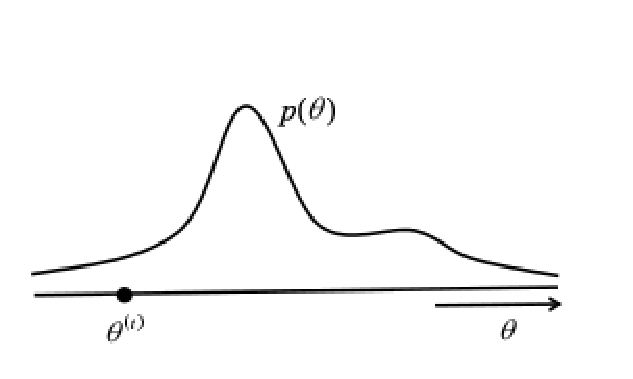
\includegraphics[width=4cm]{./ImaginiLatex/Metropolis1.eps} &
 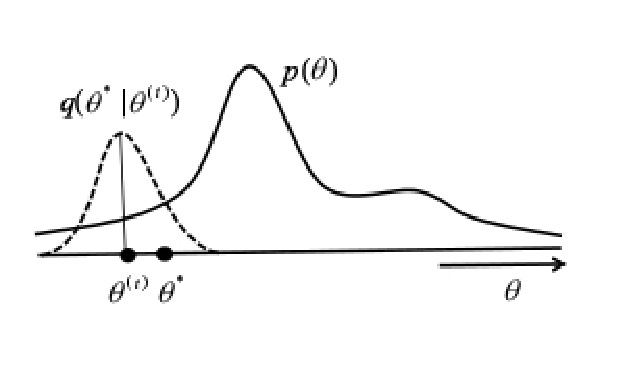
\includegraphics[width=4cm]{./ImaginiLatex/Metropolis2.eps} &
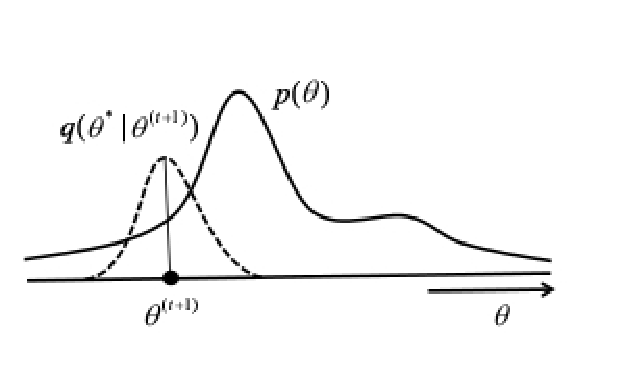
\includegraphics[width=4cm]{./ImaginiLatex/Metropolis3.eps} \\
a & b & c
\end{tabular}
\end{center}
\caption{Illustration of the Metropolis sampler to sample from target density $p(\theta)$. (a) the current state of the chain is $\theta^t$. (b) the proposal distribution $q$ around the current state is used to generate a proposal $\theta^*$ . 
(c) the proposal was accepted and the new state is set equal to the proposal, and the proposal distribution now centers on the new state.
 }
\label{fig:Metropolis}
\end{figure}

In Figure \ref{fig:Metropolis}  is illustrated how works the procedure for the generation of a sequence of two states. To intuitively understand why the process leads to samples from the target distribution, note that the method will always accept a new proposal if the the new proposal is more likely under the target distribution than the old state.
The proposal distribution is a distribution that is chosen by the researcher and good choices for the distribution depend on the problem. One important constraint for the proposal distribution is that it should cover the state space such that each potential outcome in state space has some non-zero probability under the proposal distribution 
old state. \\
Therefore, the sampler will move towards the regions of the state space where the target function has high density. However, note that if the new proposal is less likely than
than the current state, it is still possible to accept this "worse" proposal and move toward it. \\ This process of always accepting a "good" proposal, and occasionally accepting a "bad" proposal insures that the sampler explores the whole state space, and samples from all parts of a distribution (including the tails).\\
A key requirement for the Metropolis sampler is that the proposal distribution is symmetric, such that:
$$
q(\theta = \theta^t|\theta^{t-1} ) = q(\theta = \theta^{t-1} |\theta^t). 
$$
Therefore, the probability of proposing some new state given the old state, is the same as proposing to go from the new state back to the old state. This symmetry holds with proposal distributions such as the \textit{Normal, Cauchy, Student-t}, as well as \textit{Uniform} distributions. If this symmetry does not hold, you should use the Metropolis-Hastings sampler discussed in the next section.\\
A major advantage of the Metropolis sampler is that Equation \ref{eqn: Acceptance Ratio Metropolis} involves only a ratio of densities. Therefore, any terms independent of $\theta$ in the functional form of $p(\theta)$ will drop out.\\
Therefore, we do not need to know the normalizing constant of the density or probability mass function. The fact that this procedure allows us to sample from unnormalized distributions is one of its major attractions. Sampling from unnormalized distributions frequently happens in Bayesian models, where calculating the normalization constant is difficult or impractical.
\begin{example} \label{ex: Mixture of Gaussians Sampling}
In this example we try to generate random samples from a Mixture of Gaussians distribution given by:
$$
	p(\theta)=\sum_{i=1}^K \pi_i N_i(\theta | \mu_i,\sigma_i)
$$
where:
\begin{itemize}
\item $K$ is the number if components in the mixture;
\item $\pi_i$ are the mixing coefficients;
\item $N(\mu_i,\sigma_i)$ are the Gaussians components of the mixture.
\end{itemize}
Our proposals are generated from a Normal $N(\theta^t, \sigma)$ distribution. 
Therefore, the mean of the distribution is centered on the current state $\theta(t)$ and the parameter $\sigma$, which needs to be set by the modeler, controls the variability of the proposed samples.
We fixed $N=2$, $\pi=[0.3 0.5]$ , $N_1(\theta |5,4)$ , $N_2(\theta |30,3)$.
To explore the behavior of the sampling scheme we have generated different simulations varying the starting point $\theta(t_0)$ and  variability parameter $\sigma$, measuring the acceptance rate of the chain simulation.
\begin{figure}\label{fig: SimulationMetropolis0}
\begin{tabular}{cc} 
\includegraphics[width=0.5\textwidth]{ImaginiLatex/MetropolisExample1.eps} &
\includegraphics[width=0.5\textwidth]{ImaginiLatex/MetropolisExample2.eps} \\
\textbf{Simulation 1} $\theta_0=   95.33$  $\sigma=    0.25$  & \textbf{Simulation 2} $\theta_0=   70.70$  $\sigma=    0.50$
\end{tabular}
\begin{tabular}{cc} 
\includegraphics[width=0.5\textwidth]{ImaginiLatex/MetropolisExample3.eps} &
\includegraphics[width=0.5\textwidth]{ImaginiLatex/MetropolisExample4.eps} \\
\textbf{Simulation 3} $\theta_0=   95.43$  $\sigma=    0.75$  & \textbf{Simulation 4} $\theta_0=   60.22$  $\sigma=    1.00$
\end{tabular}
\begin{tabular}{cc} 
\includegraphics[width=0.5\textwidth]{ImaginiLatex/MetropolisExample5.eps} &
\includegraphics[width=0.5\textwidth]{ImaginiLatex/MetropolisExample6.eps} \\
\textbf{Simulation 5} $\theta_0=   84.23$  $\sigma=    1.25$  & \textbf{Simulation 6} $\theta_0=   44.84$  $\sigma=    1.50$
\end{tabular}
\begin{tabular}{cc} 
\includegraphics[width=0.5\textwidth]{ImaginiLatex/MetropolisExample7.eps} &
\includegraphics[width=0.5\textwidth]{ImaginiLatex/MetropolisExample8.eps} \\
\textbf{Simulation 7} $\theta_0=   83.85$  $\sigma=    1.75$  & \textbf{Simulation 8} $\theta_0=   52.35$  $\sigma=    2.00$
\end{tabular}
\caption{Simulations 1 - 8}
\end{figure}
\begin{figure}\label{fig: SimulationMetropolis1}
\begin{tabular}{cc} 
\includegraphics[width=0.5\textwidth]{ImaginiLatex/MetropolisExample9.eps} &
\includegraphics[width=0.5\textwidth]{ImaginiLatex/MetropolisExample10.eps} \\
\textbf{Simulation 9} $\theta_0=    3.20$  $\sigma=    2.25$  & \textbf{Simulation 10} $\theta_0=   38.21$  $\sigma=    2.50$
\end{tabular}
\begin{tabular}{cc} 
\includegraphics[width=0.5\textwidth]{ImaginiLatex/MetropolisExample11.eps} &
\includegraphics[width=0.5\textwidth]{ImaginiLatex/MetropolisExample12.eps} \\
\textbf{Simulation 11} $\theta_0=   89.96$  $\sigma=    2.75$  & \textbf{Simulation 12} $\theta_0=   43.47$  $\sigma=    3.00$
\end{tabular}
\begin{tabular}{cc} 
\includegraphics[width=0.5\textwidth]{ImaginiLatex/MetropolisExample13.eps} &
\includegraphics[width=0.5\textwidth]{ImaginiLatex/MetropolisExample14.eps} \\
\textbf{Simulation 13} $\theta_0=   20.76$  $\sigma=    3.25$  & \textbf{Simulation 14} $\theta_0=   31.01$  $\sigma=    3.50$
\end{tabular}
\begin{tabular}{cc} 
\includegraphics[width=0.5\textwidth]{ImaginiLatex/MetropolisExample15.eps} &
\includegraphics[width=0.5\textwidth]{ImaginiLatex/MetropolisExample16.eps} \\
\textbf{Simulation 15} $\theta_0=   54.29$  $\sigma=    3.75$  & \textbf{Simulation 16} $\theta_0=   91.11$  $\sigma=    4.00$
\end{tabular}
\caption{Simulations 2 - 16}
\end{figure}
\begin{figure}\label{fig: SimulationMetropolis2}
\begin{tabular}{cc} 
\includegraphics[width=0.5\textwidth]{ImaginiLatex/MetropolisExample17.eps} &
\includegraphics[width=0.5\textwidth]{ImaginiLatex/MetropolisExample18.eps} \\
\textbf{Simulation 17} $\theta_0=   53.00$  $\sigma=    4.25$  & \textbf{Simulation 18} $\theta_0=   31.38$  $\sigma=    4.50$
\end{tabular}
\begin{tabular}{cc} 
\includegraphics[width=0.5\textwidth]{ImaginiLatex/MetropolisExample19.eps} &
\includegraphics[width=0.5\textwidth]{ImaginiLatex/MetropolisExample20.eps} \\
\textbf{Simulation 19} $\theta_0=    4.41$  $\sigma=    4.75$  & \textbf{Simulation 20} $\theta_0=   71.82$  $\sigma=    5.00$
\end{tabular}
\begin{tabular}{cc} 
\includegraphics[width=0.5\textwidth]{ImaginiLatex/MetropolisExample21.eps} &
\includegraphics[width=0.5\textwidth]{ImaginiLatex/MetropolisExample22.eps} \\
\textbf{Simulation 21} $\theta_0=   77.10$  $\sigma=    5.25$  & \textbf{Simulation 22} $\theta_0=    6.89$  $\sigma=    5.50$
\end{tabular}
\begin{tabular}{cc} 
\includegraphics[width=0.5\textwidth]{ImaginiLatex/MetropolisExample23.eps} &
\includegraphics[width=0.5\textwidth]{ImaginiLatex/MetropolisExample24.eps} \\
\textbf{Simulation 23} $\theta_0=   63.08$  $\sigma=    5.75$  & \textbf{Simulation 24} $\theta_0=   27.25$  $\sigma=    6.00$
\end{tabular}
\caption{Simulations 3 - 24}
\end{figure}
\begin{figure}\label{fig: SimulationMetropolis3}
\begin{tabular}{cc} 
\includegraphics[width=0.5\textwidth]{ImaginiLatex/MetropolisExample25.eps} &
\includegraphics[width=0.5\textwidth]{ImaginiLatex/MetropolisExample26.eps} \\
\textbf{Simulation 25} $\theta_0=   31.92$  $\sigma=    6.25$  & \textbf{Simulation 26} $\theta_0=   52.75$  $\sigma=    6.50$
\end{tabular}
\begin{tabular}{cc} 
\includegraphics[width=0.5\textwidth]{ImaginiLatex/MetropolisExample27.eps} &
\includegraphics[width=0.5\textwidth]{ImaginiLatex/MetropolisExample28.eps} \\
\textbf{Simulation 27} $\theta_0=   41.45$  $\sigma=    6.75$  & \textbf{Simulation 28} $\theta_0=   89.40$  $\sigma=    7.00$
\end{tabular}
\begin{tabular}{cc} 
\includegraphics[width=0.5\textwidth]{ImaginiLatex/MetropolisExample29.eps} &
\includegraphics[width=0.5\textwidth]{ImaginiLatex/MetropolisExample30.eps} \\
\textbf{Simulation 29} $\theta_0=   57.80$  $\sigma=    7.25$  & \textbf{Simulation 30} $\theta_0=   57.22$  $\sigma=    7.50$
\end{tabular}
\begin{tabular}{cc} 
\includegraphics[width=0.5\textwidth]{ImaginiLatex/MetropolisExample31.eps} &
\includegraphics[width=0.5\textwidth]{ImaginiLatex/MetropolisExample32.eps} \\
\textbf{Simulation 31} $\theta_0=   40.06$  $\sigma=    7.75$  & \textbf{Simulation 32} $\theta_0=   69.47$  $\sigma=    8.00$
\end{tabular}
\caption{Simulations 4 - 32}
\end{figure}
\begin{figure}\label{fig: SimulationMetropolis4}
\begin{tabular}{cc} 
\includegraphics[width=0.5\textwidth]{ImaginiLatex/MetropolisExample33.eps} &
\includegraphics[width=0.5\textwidth]{ImaginiLatex/MetropolisExample34.eps} \\
\textbf{Simulation 33} $\theta_0=   57.36$  $\sigma=    8.25$  & \textbf{Simulation 34} $\theta_0=   34.98$  $\sigma=    8.50$
\end{tabular}
\begin{tabular}{cc} 
\includegraphics[width=0.5\textwidth]{ImaginiLatex/MetropolisExample35.eps} &
\includegraphics[width=0.5\textwidth]{ImaginiLatex/MetropolisExample36.eps} \\
\textbf{Simulation 35} $\theta_0=   59.90$  $\sigma=    8.75$  & \textbf{Simulation 36} $\theta_0=   28.12$  $\sigma=    9.00$
\end{tabular}
\end{figure}

Figure \ref{fig:SimulationMetropolis0} - \ref{fig:SimulationMetropolis4} show the simulation results for the different chains run for $500$ iterations.
The upper panel shows the theoretical density in the dashed red line and the histogram shows the distribution of all $500$ samples. The lower panel shows the sequence of samples of one chain.\\
Table \ref{tab: Simulation Metropolis} reports the acceptance ratio for each simulation.\\
\begin{center}
\begin{table}\label{tb: Simulation Metropolis}
\begin{tabular}{|ccccc|}\hline 
Simulation & $\theta_0$ & $\sigma$ & Acceptance ratio & Reject ratio)\\ \hline 
1 &    95.33 &     0.25 &     0.52 &     0.48 \\  \hline 
2 &    70.70 &     0.50 &     0.48 &     0.52 \\  
3 &    95.43 &     0.75 &     0.47 &     0.53 \\  
4 &    60.22 &     1.00 &     0.49 &     0.51 \\  
5 &    84.23 &     1.25 &     0.48 &     0.52 \\  
6 &    44.84 &     1.50 &     0.49 &     0.51 \\  
7 &    83.85 &     1.75 &     0.49 &     0.51 \\  
8 &    52.35 &     2.00 &     0.46 &     0.54 \\  
9 &     3.20 &     2.25 &     0.47 &     0.53 \\  
10 &    38.21 &     2.50 &     0.47 &     0.53 \\  
11 &    89.96 &     2.75 &     0.43 &     0.57 \\  
12 &    43.47 &     3.00 &     0.52 &     0.48 \\  
13 &    20.76 &     3.25 &     0.46 &     0.54 \\  
14 &    31.01 &     3.50 &     0.46 &     0.54 \\  
15 &    54.29 &     3.75 &     0.44 &     0.56 \\  
16 &    91.11 &     4.00 &     0.42 &     0.58 \\  
17 &    53.00 &     4.25 &     0.46 &     0.54 \\  
18 &    31.38 &     4.50 &     0.44 &     0.56 \\  
19 &     4.41 &     4.75 &     0.43 &     0.57 \\  
20 &    71.82 &     5.00 &     0.43 &     0.57 \\  
21 &    77.10 &     5.25 &     0.41 &     0.59 \\  
22 &     6.89 &     5.50 &     0.38 &     0.62 \\  
23 &    63.08 &     5.75 &     0.41 &     0.59 \\  
24 &    27.25 &     6.00 &     0.42 &     0.58 \\  
25 &    31.92 &     6.25 &     0.40 &     0.60 \\  
26 &    52.75 &     6.50 &     0.39 &     0.61 \\  
27 &    41.45 &     6.75 &     0.39 &     0.61 \\  
28 &    89.40 &     7.00 &     0.39 &     0.61 \\  
29 &    57.80 &     7.25 &     0.34 &     0.66 \\  
30 &    57.22 &     7.50 &     0.36 &     0.64 \\  
31 &    40.06 &     7.75 &     0.38 &     0.62 \\  
32 &    69.47 &     8.00 &     0.37 &     0.63 \\  
33 &    57.36 &     8.25 &     0.36 &     0.64 \\  
34 &    34.98 &     8.50 &     0.37 &     0.63 \\  
35 &    59.90 &     8.75 &     0.33 &     0.67 \\  
36 &    28.12 &     9.00 &     0.34 &     0.66 \\  
\end{tabular}
\caption{ Metropolis simulation results varying $\theta_0$ and $\sigma$ }
\end{table}
\end{center}



\end{example}

\newpage

\section{Metropolis-Hasting sampler}
The Metropolis-Hasting (\textbf{MH}) sampler is a generalized version of the Metropolis sampler in which we can apply symmetric as well as asymmetric proposal distributions. The \textbf{MH} sampler operates in exactly the same fashion as the Metropolis sampler, but uses the following acceptance probability: 
\begin{eqnarray} \label{eqn: Acceptance Ratio MH}
\alpha = min(1, \frac{p(\theta^*)}{p(\theta^{t-1})} \frac{q(\theta^{t-1}|\theta^∗) }{q(\theta^∗ |\theta^{t-1})}
\end{eqnarray}

The additional ratio $\frac{q(\theta^{t-1}|\theta^∗)}{q(\theta^∗ |\theta^{t-1})}$ in  \ref{eqn: Acceptance Ratio MH} corrects for any asymmetries in the proposal distribution. For example, suppose we have a proposal distribution with a mean centered on the current state, but that is skewed in one direction. If the proposal distribution prefers to move say left over right, the proposal density ratio will correct for this asymmetry.
We can summarize the \textbf{MH} sampler in the following operations:\\
{\bf METROPOLIS Sampler}\\[.4cm]
{\sf
0. \hspace*{0.2cm} Set $t=1$  \\
1. \hspace*{0.2cm} Generate a initial value $u$, and set $\theta^1 = u$\\
2. \hspace*{0.2cm}  Repeat\\
2.1 \hspace*{0.3cm} $t=t+1$\\
2.2 \hspace*{0.3cm} generate a candidate point $\theta^∗$ from proposal distribution:
$$
\theta^∗ \approx q(\theta^t |\theta^{t-1})
$$
2.3 \hspace*{0.3cm} calculate acceptance probability \\
$$
\alpha = min(1, \frac{p(\theta^*)}{p(\theta^{t-1})} \frac{q(\theta^{t-1}|\theta^∗)}{q(\theta^∗ |\theta^{t-1})} )
$$
2.4 \hspace*{0.3cm} generate $u$ from Uniform distribution in $[0 1]$\\
2.5 \hspace*{0.3cm} if($\alpha  \leq u$)\\
2.6 \hspace*{0.4cm}  \textbf{accept sample}: $\theta^t=\theta^∗$.\\
2.7 \hspace*{0.3cm} else\\
2.8 \hspace*{0.4cm}  \textbf{reject sample}: $\theta^t=\theta^{t-1}$.\\
3. \hspace*{0.2cm} Until $t = T$\\
}\\[.4cm]
\\
\\
The fact that asymmetric proposal distributions can be used allows the Metropolis-Hastings procedure to sample from target distributions that are defined on a limited range
(other than the uniform for which Metropolis sampler can be used). With bounded variables, care should be taken in constructing a suitable proposal distribution. Generally, a
good rule is to use a proposal distribution has positive density on the same support as the
target distribution.
\begin{example} \label{ex: Mixture of Gaussians Sampling 2}
In this example we try to generate random samples from the target distribution (\textbf{MOG}) discussed in example \ref{ex: Mixture of Gaussians Sampling}  using as proposal the Gamma distribution:
$$
q(\theta^t|\theta(t-1))= Gamma(\theta^t| \theta^{t-1} * \tau , frac{1}{\tau})
$$
This proposal density has a mean equal to $\theta^t$ so it is \"centered\" on the current state. The parameter $\tau$ is a precision parameter controlling the acceptance rate of the sampler so that higher values are associated with less variability in the proposal distribution.
\begin{figure}\label{fig: SimulationMetropolisHasting0}
\begin{tabular}{cc} 
\includegraphics[width=0.5\textwidth]{ImaginiLatex/MetropolisExample1.eps} &
\includegraphics[width=0.5\textwidth]{ImaginiLatex/MetropolisExample2.eps} \\
\textbf{Simulation 1} $\theta_0=   95.33$  $\tau=    0.25$  & \textbf{Simulation 2} $\theta_0=   70.70$  $\tau=    0.50$
\end{tabular}
\begin{tabular}{cc} 
\includegraphics[width=0.5\textwidth]{ImaginiLatex/MetropolisExample3.eps} &
\includegraphics[width=0.5\textwidth]{ImaginiLatex/MetropolisExample4.eps} \\
\textbf{Simulation 3} $\theta_0=   95.43$  $\tau=    0.75$  & \textbf{Simulation 4} $\theta_0=   60.22$  $\tau=    1.00$
\end{tabular}
\begin{tabular}{cc} 
\includegraphics[width=0.5\textwidth]{ImaginiLatex/MetropolisExample5.eps} &
\includegraphics[width=0.5\textwidth]{ImaginiLatex/MetropolisExample6.eps} \\
\textbf{Simulation 5} $\theta_0=   84.23$  $\tau=    1.25$  & \textbf{Simulation 6} $\theta_0=   44.84$  $\tau=    1.50$
\end{tabular}
\begin{tabular}{cc} 
\includegraphics[width=0.5\textwidth]{ImaginiLatex/MetropolisExample7.eps} &
\includegraphics[width=0.5\textwidth]{ImaginiLatex/MetropolisExample8.eps} \\
\textbf{Simulation 7} $\theta_0=   83.85$  $\tau=    1.75$  & \textbf{Simulation 8} $\theta_0=   52.35$  $\tau=    2.00$
\end{tabular}
\caption{Simulations 1 - 8}
\end{figure}
\begin{figure}\label{fig: SimulationMetropolisHasting1}
\begin{tabular}{cc} 
\includegraphics[width=0.5\textwidth]{ImaginiLatex/MetropolisExample9.eps} &
\includegraphics[width=0.5\textwidth]{ImaginiLatex/MetropolisExample10.eps} \\
\textbf{Simulation 9} $\theta_0=    3.20$  $\tau=    2.25$  & \textbf{Simulation 10} $\theta_0=   38.21$  $\tau=    2.50$
\end{tabular}
\begin{tabular}{cc} 
\includegraphics[width=0.5\textwidth]{ImaginiLatex/MetropolisExample11.eps} &
\includegraphics[width=0.5\textwidth]{ImaginiLatex/MetropolisExample12.eps} \\
\textbf{Simulation 11} $\theta_0=   89.96$  $\tau=    2.75$  & \textbf{Simulation 12} $\theta_0=   43.47$  $\tau=    3.00$
\end{tabular}
\begin{tabular}{cc} 
\includegraphics[width=0.5\textwidth]{ImaginiLatex/MetropolisExample13.eps} &
\includegraphics[width=0.5\textwidth]{ImaginiLatex/MetropolisExample14.eps} \\
\textbf{Simulation 13} $\theta_0=   20.76$  $\tau=    3.25$  & \textbf{Simulation 14} $\theta_0=   31.01$  $\tau=    3.50$
\end{tabular}
\begin{tabular}{cc} 
\includegraphics[width=0.5\textwidth]{ImaginiLatex/MetropolisExample15.eps} &
\includegraphics[width=0.5\textwidth]{ImaginiLatex/MetropolisExample16.eps} \\
\textbf{Simulation 15} $\theta_0=   54.29$  $\tau=    3.75$  & \textbf{Simulation 16} $\theta_0=   91.11$  $\tau=    4.00$
\end{tabular}
\caption{Simulations 2 - 16}
\end{figure}
\begin{figure}\label{fig: SimulationMetropolisHasting2}
\begin{tabular}{cc} 
\includegraphics[width=0.5\textwidth]{ImaginiLatex/MetropolisExample17.eps} &
\includegraphics[width=0.5\textwidth]{ImaginiLatex/MetropolisExample18.eps} \\
\textbf{Simulation 17} $\theta_0=   53.00$  $\tau=    4.25$  & \textbf{Simulation 18} $\theta_0=   31.38$  $\tau=    4.50$
\end{tabular}
\begin{tabular}{cc} 
\includegraphics[width=0.5\textwidth]{ImaginiLatex/MetropolisExample19.eps} &
\includegraphics[width=0.5\textwidth]{ImaginiLatex/MetropolisExample20.eps} \\
\textbf{Simulation 19} $\theta_0=    4.41$  $\tau=    4.75$  & \textbf{Simulation 20} $\theta_0=   71.82$  $\tau=    5.00$
\end{tabular}
\begin{tabular}{cc} 
\includegraphics[width=0.5\textwidth]{ImaginiLatex/MetropolisExample21.eps} &
\includegraphics[width=0.5\textwidth]{ImaginiLatex/MetropolisExample22.eps} \\
\textbf{Simulation 21} $\theta_0=   77.10$  $\tau=    5.25$  & \textbf{Simulation 22} $\theta_0=    6.89$  $\tau=    5.50$
\end{tabular}
\begin{tabular}{cc} 
\includegraphics[width=0.5\textwidth]{ImaginiLatex/MetropolisExample23.eps} &
\includegraphics[width=0.5\textwidth]{ImaginiLatex/MetropolisExample24.eps} \\
\textbf{Simulation 23} $\theta_0=   63.08$  $\tau=    5.75$  & \textbf{Simulation 24} $\theta_0=   27.25$  $\tau=    6.00$
\end{tabular}
\caption{Simulations 3 - 24}
\end{figure}
\begin{figure}\label{fig: SimulationMetropolisHasting3}
\begin{tabular}{cc} 
\includegraphics[width=0.5\textwidth]{ImaginiLatex/MetropolisExample25.eps} &
\includegraphics[width=0.5\textwidth]{ImaginiLatex/MetropolisExample26.eps} \\
\textbf{Simulation 25} $\theta_0=   31.92$  $\tau=    6.25$  & \textbf{Simulation 26} $\theta_0=   52.75$  $\tau=    6.50$
\end{tabular}
\begin{tabular}{cc} 
\includegraphics[width=0.5\textwidth]{ImaginiLatex/MetropolisExample27.eps} &
\includegraphics[width=0.5\textwidth]{ImaginiLatex/MetropolisExample28.eps} \\
\textbf{Simulation 27} $\theta_0=   41.45$  $\tau=    6.75$  & \textbf{Simulation 28} $\theta_0=   89.40$  $\tau=    7.00$
\end{tabular}
\begin{tabular}{cc} 
\includegraphics[width=0.5\textwidth]{ImaginiLatex/MetropolisExample29.eps} &
\includegraphics[width=0.5\textwidth]{ImaginiLatex/MetropolisExample30.eps} \\
\textbf{Simulation 29} $\theta_0=   57.80$  $\tau=    7.25$  & \textbf{Simulation 30} $\theta_0=   57.22$  $\tau=    7.50$
\end{tabular}
\begin{tabular}{cc} 
\includegraphics[width=0.5\textwidth]{ImaginiLatex/MetropolisExample31.eps} &
\includegraphics[width=0.5\textwidth]{ImaginiLatex/MetropolisExample32.eps} \\
\textbf{Simulation 31} $\theta_0=   40.06$  $\tau=    7.75$  & \textbf{Simulation 32} $\theta_0=   69.47$  $\tau=    8.00$
\end{tabular}
\caption{Simulations 4 - 32}
\end{figure}
\begin{figure}\label{fig: SimulationMetropolisHasting4}
\begin{tabular}{cc} 
\includegraphics[width=0.5\textwidth]{ImaginiLatex/MetropolisExample33.eps} &
\includegraphics[width=0.5\textwidth]{ImaginiLatex/MetropolisExample34.eps} \\
\textbf{Simulation 33} $\theta_0=   57.36$  $\tau=    8.25$  & \textbf{Simulation 34} $\theta_0=   34.98$  $\tau=    8.50$
\end{tabular}
\begin{tabular}{cc} 
\includegraphics[width=0.5\textwidth]{ImaginiLatex/MetropolisExample35.eps} &
\includegraphics[width=0.5\textwidth]{ImaginiLatex/MetropolisExample36.eps} \\
\textbf{Simulation 35} $\theta_0=   59.90$  $\tau=    8.75$  & \textbf{Simulation 36} $\theta_0=   28.12$  $\tau=    9.00$
\end{tabular}
\end{figure}

In figures \ref{fig:SimulationMetropolisHasting0} - \ref{fig:SimulationMetropolisHasting4} are depicted the simulation results for different chains runs for $500$ iterations.
Again, in the upper panel are depicted the theoretical density in the dashed red line and the distribution of all $500$ generated samples, while in the lower panel is showed the sequence in time of generated samples (rejected and accepted samples).\\
In table ~\ref{tab: Simulation Metropolis} we report the acceptance ratio for each simulation.\\
\begin{center}
\begin{table}\label{tb: Simulation Metropolis}
\begin{tabular}{|ccccc|}\hline 
Simulation & $\theta_0$ & $\sigma$ & Acceptance ratio & Reject ratio)\\ \hline 
1 &    95.33 &     0.25 &     0.38 &     0.62 \\  \hline 
2 &    70.70 &     0.50 &     0.42 &     0.58 \\  
3 &    95.43 &     0.75 &     0.47 &     0.53 \\  
4 &    60.22 &     1.00 &     0.53 &     0.47 \\  
5 &    84.23 &     1.25 &     0.51 &     0.49 \\  
6 &    44.84 &     1.50 &     0.50 &     0.50 \\  
7 &    83.85 &     1.75 &     0.61 &     0.39 \\  
8 &    52.35 &     2.00 &     0.60 &     0.40 \\  
9 &     3.20 &     2.25 &     0.61 &     0.39 \\  
10 &    38.21 &     2.50 &     0.61 &     0.39 \\  
11 &    89.96 &     2.75 &     0.66 &     0.34 \\  
12 &    43.47 &     3.00 &     0.70 &     0.30 \\  
13 &    20.76 &     3.25 &     0.73 &     0.27 \\  
14 &    31.01 &     3.50 &     0.64 &     0.36 \\  
15 &    54.29 &     3.75 &     0.70 &     0.30 \\  
16 &    91.11 &     4.00 &     0.69 &     0.31 \\  
17 &    53.00 &     4.25 &     0.73 &     0.27 \\  
18 &    31.38 &     4.50 &     0.78 &     0.22 \\  
19 &     4.41 &     4.75 &     0.72 &     0.28 \\  
20 &    71.82 &     5.00 &     0.71 &     0.29 \\  
21 &    77.10 &     5.25 &     0.74 &     0.26 \\  
22 &     6.89 &     5.50 &     0.71 &     0.29 \\  
23 &    63.08 &     5.75 &     0.76 &     0.24 \\  
24 &    27.25 &     6.00 &     0.75 &     0.25 \\  
25 &    31.92 &     6.25 &     0.80 &     0.20 \\  
26 &    52.75 &     6.50 &     0.75 &     0.25 \\  
27 &    41.45 &     6.75 &     0.71 &     0.29 \\  
28 &    89.40 &     7.00 &     0.71 &     0.29 \\  
29 &    57.80 &     7.25 &     0.77 &     0.23 \\  
30 &    57.22 &     7.50 &     0.70 &     0.30 \\  
31 &    40.06 &     7.75 &     0.80 &     0.20 \\  
32 &    69.47 &     8.00 &     0.72 &     0.28 \\  
33 &    57.36 &     8.25 &     0.74 &     0.26 \\  
34 &    34.98 &     8.50 &     0.79 &     0.21 \\  
35 &    59.90 &     8.75 &     0.76 &     0.24 \\  
36 &    28.12 &     9.00 &     0.88 &     0.12 \\  
\end{tabular}
\caption{ Metropolis simulation results varying $\theta_0$ and $\sigma$ }
\end{table}
\end{center}

\end{example}
\newpage
\subsection{Metropolis-Hastings for Multivariate Distributions}
The generalization of MH sampler to multivariate distributions can be obtained following two different approaches differing each other in the strategy used to explore multidimensional spaces, namely blockwise or componentwise upadating.
Let $\mathbf{\theta} = (\theta_1, \theta_2 , . . . ,\theta_N )$ be a random variable involving $N$ components, our objective is to generate a chain:
$$
\mathbf{\theta^1}  \rightarrow  \mathbf{\theta^2}  \rightarrow . .  \rightarrow  \mathbf{\theta^t}  \rightarrow . . .
$$
where  $\mathbf{\theta^t}$ represents the N-dimensional sample generated at time $t$.

\subsubsection{Blockwise updating}
The blockwise updating approach uses a proposal distribution having same dimensionality as the target distribution. So, if we want to sample from a probability distribution involving $N$ variables, we design a N-dimensional proposal distribution, and we either accept or reject the proposal (involving values for all $N$ variables) as a block.\\
This leads to a generalization of the \textbf{MH} sampler where the scalar samples $\theta^t$ are now replaced by vectors $\mathbf{\theta^t}$:\\
{\bf METROPOLIS HASTING B.W}\\[.4cm]
{\sf
0. \hspace*{0.2cm} Set $t=1$  \\
1. \hspace*{0.2cm} Generate a initial value $\mathbf{\theta^1}=(\theta_1^1, \theta_2^1 , . . . ,\theta_N^1 )$\
2. \hspace*{0.2cm}  Repeat\\
2.1 \hspace*{0.3cm} $t=t+1$\\
2.2 \hspace*{0.3cm} generate a candidate point $\theta^∗$ from proposal distribution:\\
$$
\mathbf{\theta^∗} \approx q(\mathbf{\theta^t}|\mathbf{ \theta^{t-1} })
$$
2.3 \hspace*{0.3cm} calculate acceptance probability \\
$$
\alpha = min(1, \frac{p(\mathbf{\theta^*})}{p(\mathbf{\theta^{t-1}})} \frac{q(\mathbf{\theta^{t-1}}|\mathbf{\theta^∗})}{q(\mathbf{\theta^∗} |\mathbf{\theta^{t-1}})} )
$$
2.4 \hspace*{0.3cm} generate $u$ from Uniform distribution in $[0 1]$\\
2.5 \hspace*{0.3cm} if($\alpha  \leq u$)\\
\hspace*{0.4cm}  \textbf{accept sample}: $\theta^t=\theta^∗$.\\
\hspace*{0.3cm} else\\
\hspace*{0.4cm}  \textbf{reject sample}: $\theta^t=\theta^{t-1}$.\\
3. \hspace*{0.2cm} Until $t = T$\\
}\\[.4cm]
\\
\\
A potential problem with the blockwise updating approach is that it might be difficult to
find suitable high-dimensional proposal distributions. A related problem is that blockwise
updating can be associated with high rejection rates. 
\subsubsection{Componentwise updating}
Instead of accepting or rejecting a proposal for $\theta$ involving all its components simultaneously, the component wise approach generate proposal for individual components of $\theta$, once per time.\\
This leads to a  computationally simpler updating approach where at each iteration $t$, we  make an independent proposal $\theta_i^*$ for each component status $\theta_i^t$ given its previous state  $\theta_i^{t-1}$ and evaluate the acceptance ratio comparing the likelihood of $(\theta_i^* , \theta_{j\neq i}^{t-1} )$ against $(\theta_i^{t-1} , \theta_{j\neq i}^{t-1} )$.
Note that in this proposal procedure, we  vary at each time only one component keeping the others component constant and updated to the last generated proposal.  Therefore, what happens while proposing a new sample for $\theta_{j}^{t}$ is conditioned on what
happened in proposal generation for all components $i<j$ .
The whole procedure is summarized in the following steps:\\

{\bf METROPOLIS-HASTING C.W. }\\[.4cm]
{\sf
0. \hspace*{0.2cm} Set $t=1$  \\
1. \hspace*{0.2cm} Generate a initial value $\mathbf{\theta^1}=(\theta_1^1, \theta_2^1 , . . . ,\theta_N^1 )$\\
2. \hspace*{0.2cm}  Repeat\\
2.1 \hspace*{0.3cm} $t=t+1$\\
2.2 \hspace*{0.3cm}  For $i=1:N$\\
2.2 \hspace*{0.4cm} generate a candidate component $\theta_i^∗$ from proposal distribution:
$$
\theta_i^∗ \approx q( \theta_i^t |\theta_i^{t-1} )
$$
3.3 \hspace*{0.4cm} calculate acceptance probability \\
$$
\alpha = min(1, \frac{p(\theta_i^*,\theta_{j \neq i}^{t-1})}{p(\mathbf{\theta^{t-1}})} \frac{q( \theta_i^{t-1}| \theta_i^{∗} ) } { q( \theta_i^{∗}| \theta_i^{t-1} )} )
$$
2.4 \hspace*{0.4cm} generate $u$ from Uniform distribution in $[0 1]$\\
2.4 \hspace*{0.4cm} if($\alpha  \leq u$)\\
2.5 \hspace*{0.5cm}  \textbf{accept sample component}: $\theta_i^t=\theta_i^∗$.\\
2.6 \hspace*{0.4cm} else\\
2.7 \hspace*{0.5cm}  \textbf{reject sample component}: $\theta_i^t=\theta_i^{t-1}$.\\
2.8 \hspace*{0.3cm}  EndFor \\
3.\hspace*{0.2cm} Until $t = T$\\
}\\[.4cm]
\\
\\
\begin{example} \label{ex: Mixture of Multivariate Gaussians Sampling}
In this example we try to generate random samples from a Mixture of multivariate Gaussians distribution given by:
$$
	p(\theta)=\sum_{i=1}^K \pi(i)N_i(\theta | \mu_i,\Sigma_i)
$$
where:
\begin{itemize}
\item $K$ is the number if components in the mixture;
\item $\pi_i$ are the mixing coefficients;
\item $N(\mu_i,\Sigma_i)$ are the multivariate Gaussians components of the mixture 
parametrized by the mean vector $1 \times N \mu$ and the covariance matrix
$N \times N \Sigma$
\end{itemize}
We used as proposal the Gamma distribution described in \ref{ex: Mixture of Gaussians Sampling 2}
We fixed $N=2$, $\pi=[0.3 0.5]$ , $N_1(\theta |5,4)$ , $N_2(\theta |30,3)$.
To explore the behavior of the sampling scheme we have generated different simulations varying the starting point $\theta(t_0)$ and the Gamma distribution parameters , measuring the acceptance rate of each chain simulation. In table ~\ref{tab: Simulation Metropolis} are reported obtained result.
\begin{center}
\begin{table}\label{tb: Simulation Metropolis}
\begin{tabular}{|cccccc|}\hline 
Simulation & $\theta_0$ & $a$ & $b$ & Acceptance ratio & Reject ratio)\\ \hline 
1 & (    5.00 ,     5.00) &     0.10 &     1.00 &     1.00 &     0.00 \\  \hline\hline 
2 & (    5.00 ,     5.00) &     0.10 &     2.00 &     0.98 &     0.02 \\  \hline
3 & (    5.00 ,     5.00) &     0.10 &     3.00 &     1.00 &     0.00 \\  \hline
4 & (    5.00 ,     5.00) &     0.10 &     4.00 &     0.77 &     0.23 \\  \hline
5 & (    5.00 ,     5.00) &     0.57 &     1.00 &     0.92 &     0.08 \\  \hline
6 & (    5.00 ,     5.00) &     0.57 &     2.00 &     0.38 &     0.62 \\  \hline
7 & (    5.00 ,     5.00) &     0.57 &     3.00 &     0.08 &     0.92 \\  \hline
8 & (    5.00 ,     5.00) &     0.57 &     4.00 &     0.01 &     0.99 \\  \hline
9 & (    5.00 ,     5.00) &     1.03 &     2.00 &     0.01 &     0.99 \\  \hline
10 & (    5.00 ,     5.00) &     1.03 &     3.00 &     0.00 &     1.00 \\  \hline
11 & (    5.00 ,     5.00) &     1.03 &     4.00 &     0.00 &     1.00 \\  \hline
12 & (    5.00 ,     5.00) &     1.50 &     2.00 &     0.00 &     1.00 \\  \hline
13 & (    5.00 ,     5.00) &     1.50 &     3.00 &     0.94 &     0.06 \\  \hline
14 & (    5.00 ,     5.00) &     1.50 &     4.00 &     1.00 &     0.00 \\  \hline
15 & (   11.67 ,    11.67) &     0.10 &     1.00 &     1.00 &     0.00 \\  \hline
16 & (   11.67 ,    11.67) &     0.10 &     2.00 &     0.94 &     0.06 \\  \hline
17 & (   11.67 ,    11.67) &     0.10 &     3.00 &     0.97 &     0.03 \\  \hline
18 & (   11.67 ,    11.67) &     0.10 &     4.00 &     0.73 &     0.27 \\  \hline
19 & (   11.67 ,    11.67) &     0.57 &     1.00 &     0.97 &     0.03 \\  \hline
20 & (   11.67 ,    11.67) &     0.57 &     2.00 &     0.41 &     0.59 \\  \hline
21 & (   11.67 ,    11.67) &     0.57 &     3.00 &     0.05 &     0.95 \\  \hline
22 & (   11.67 ,    11.67) &     0.57 &     4.00 &     0.01 &     0.99 \\  \hline
23 & (   11.67 ,    11.67) &     1.03 &     2.00 &     0.00 &     1.00 \\  \hline
24 & (   11.67 ,    11.67) &     1.03 &     3.00 &     0.00 &     1.00 \\  \hline
25 & (   11.67 ,    11.67) &     1.03 &     4.00 &     0.00 &     1.00 \\  \hline
26 & (   11.67 ,    11.67) &     1.50 &     2.00 &     0.00 &     1.00 \\  \hline
27 & (   11.67 ,    11.67) &     1.50 &     3.00 &     0.98 &     0.02 \\  \hline
28 & (   11.67 ,    11.67) &     1.50 &     4.00 &     0.99 &     0.01 \\  \hline
29 & (   18.33 ,    18.33) &     0.10 &     1.00 &     1.00 &     0.00 \\  \hline
30 & (   18.33 ,    18.33) &     0.10 &     2.00 &     0.97 &     0.03 \\  \hline
31 & (   18.33 ,    18.33) &     0.10 &     3.00 &     0.94 &     0.06 \\  \hline
32 & (   18.33 ,    18.33) &     0.10 &     4.00 &     0.82 &     0.18 \\  \hline
33 & (   18.33 ,    18.33) &     0.57 &     1.00 &     0.95 &     0.05 \\  \hline
34 & (   18.33 ,    18.33) &     0.57 &     2.00 &     0.40 &     0.60 \\  \hline
35 & (   18.33 ,    18.33) &     0.57 &     3.00 &     0.06 &     0.94 \\  \hline
36 & (   18.33 ,    18.33) &     0.57 &     4.00 &     0.01 &     0.99 \\  \hline
37 & (   18.33 ,    18.33) &     1.03 &     2.00 &     0.00 &     1.00 \\  \hline
38 & (   18.33 ,    18.33) &     1.03 &     3.00 &     0.00 &     1.00 \\  \hline
39 & (   18.33 ,    18.33) &     1.03 &     4.00 &     0.00 &     1.00 \\  \hline
40 & (   18.33 ,    18.33) &     1.50 &     2.00 &     0.00 &     1.00 \\  \hline
41 & (   18.33 ,    18.33) &     1.50 &     3.00 &     0.46 &     0.54 \\  \hline
42 & (   18.33 ,    18.33) &     1.50 &     4.00 &     0.93 &     0.07 \\  \hline
43 & (   25.00 ,    25.00) &     0.10 &     1.00 &     0.99 &     0.01 \\  \hline
44 & (   25.00 ,    25.00) &     0.10 &     2.00 &     0.97 &     0.03 \\  \hline
45 & (   25.00 ,    25.00) &     0.10 &     3.00 &     0.97 &     0.03 \\  \hline
46 & (   25.00 ,    25.00) &     0.10 &     4.00 &     0.98 &     0.02 \\  \hline
47 & (   25.00 ,    25.00) &     0.57 &     1.00 &     0.95 &     0.05 \\  \hline
48 & (   25.00 ,    25.00) &     0.57 &     2.00 &     0.37 &     0.63 \\  \hline
49 & (   25.00 ,    25.00) &     0.57 &     3.00 &     0.07 &     0.94 \\  \hline
50 & (   25.00 ,    25.00) &     0.57 &     4.00 &     0.01 &     0.99 \\  \hline
51 & (   25.00 ,    25.00) &     1.03 &     2.00 &     0.00 &     1.00 \\  \hline
52 & (   25.00 ,    25.00) &     1.03 &     3.00 &     0.00 &     1.00 \\  \hline
53 & (   25.00 ,    25.00) &     1.03 &     4.00 &     0.00 &     1.00 \\  \hline
54 & (   25.00 ,    25.00) &     1.50 &     2.00 &     0.00 &     1.00 \\  \hline
55 & (   25.00 ,    25.00) &     1.50 &     3.00 &     0.00 &     1.00 \\  \hline
56 & (   25.00 ,    25.00) &     1.50 &     4.00 &     0.98 &     0.02 \\  \hline
\end{tabular}
\caption{ Metropolis simulation results varying $\theta_0$ and $\sigma$ }
\end{table}
\end{center}

Reported results underline a typical drawback of the Metropolis-Hastings scheme and in general of rejection samplers: the difficulties
in tuning the proposal distribution to avoid production of rejected samples that are no used in approximation process. 
In figures \ref{fig:SimulationMetropolisHasting0} - \ref{fig:SimulationMetropolisHasting4} are showed the simulation results for different chains runs for $500$ iterations:  in the upper panel is depicted the histogram of generated samples, while in the lower panel are showed the isolines of the sampled distribution and the sequence of generated samples . The green point correspond to the starting sample, the blue point is the last generated sample while the red ones are samples generated during the simulation.\\
Again, the simulation shows how could be difficult to tune the proposal distribution.
\centering
\begin{figure}\label{fig: SimulationMetropolisHasting0}
\begin{tabular}{cc} 
\includegraphics[width=0.5\textwidth]{ImaginiLatex/MetropolisHastingCWExample1.eps} &
\includegraphics[width=0.5\textwidth]{ImaginiLatex/MetropolisHastingCWExample2.eps} \\
\textbf{Simulation 1} $\theta_0=(    5.00,     5.00)$  $(a,b)=(    0.10,    1.00)$  & \textbf{Simulation 2} $\theta_0=(    5.00,     5.00)$  $(a,b)=(    0.10,    2.00)$
\end{tabular}
\begin{tabular}{cc} 
\includegraphics[width=0.5\textwidth]{ImaginiLatex/MetropolisHastingCWExample3.eps} &
\includegraphics[width=0.5\textwidth]{ImaginiLatex/MetropolisHastingCWExample4.eps} \\
\textbf{Simulation 3} $\theta_0=(    5.00,     5.00)$  $(a,b)=(    0.10,    3.00)$  & \textbf{Simulation 4} $\theta_0=(    5.00,     5.00)$  $(a,b)=(    0.10,    4.00)$
\end{tabular}
\begin{tabular}{cc} 
\includegraphics[width=0.5\textwidth]{ImaginiLatex/MetropolisHastingCWExample5.eps} &
\includegraphics[width=0.5\textwidth]{ImaginiLatex/MetropolisHastingCWExample6.eps} \\
\textbf{Simulation 5} $\theta_0=(    5.00,     5.00)$  $(a,b)=(    0.57,    1.00)$  & \textbf{Simulation 6} $\theta_0=(    5.00,     5.00)$  $(a,b)=(    0.57,    2.00)$
\end{tabular}
\begin{tabular}{cc} 
\includegraphics[width=0.5\textwidth]{ImaginiLatex/MetropolisHastingCWExample7.eps} &
\includegraphics[width=0.5\textwidth]{ImaginiLatex/MetropolisHastingCWExample8.eps} \\
\textbf{Simulation 7} $\theta_0=(    5.00,     5.00)$  $(a,b)=(    0.57,    3.00)$  & \textbf{Simulation 8} $\theta_0=(    5.00,     5.00)$  $(a,b)=(    0.57,    4.00)$
\end{tabular}
\caption{Simulations 1 - 8}
\end{figure}
\begin{figure}\label{fig: SimulationMetropolisHastingCW1}
\begin{tabular}{cc} 
\includegraphics[width=0.5\textwidth]{ImaginiLatex/MetropolisHastingCWExample9.eps} &
\includegraphics[width=0.5\textwidth]{ImaginiLatex/MetropolisHastingCWExample10.eps} \\
\textbf{Simulation 9} $\theta_0=(    5.00,     5.00)$  $(a,b)=(    1.03,    2.00)$  & \textbf{Simulation 10} $\theta_0=(    5.00,     5.00)$  $(a,b)=(    1.03,    3.00)$
\end{tabular}
\begin{tabular}{cc} 
\includegraphics[width=0.5\textwidth]{ImaginiLatex/MetropolisHastingCWExample11.eps} &
\includegraphics[width=0.5\textwidth]{ImaginiLatex/MetropolisHastingCWExample12.eps} \\
\textbf{Simulation 11} $\theta_0=(    5.00,     5.00)$  $(a,b)=(    1.03,    4.00)$  & \textbf{Simulation 12} $\theta_0=(    5.00,     5.00)$  $(a,b)=(    1.50,    2.00)$
\end{tabular}
\begin{tabular}{cc} 
\includegraphics[width=0.5\textwidth]{ImaginiLatex/MetropolisHastingCWExample13.eps} &
\includegraphics[width=0.5\textwidth]{ImaginiLatex/MetropolisHastingCWExample14.eps} \\
\textbf{Simulation 13} $\theta_0=(    5.00,     5.00)$  $(a,b)=(    1.50,    3.00)$  & \textbf{Simulation 14} $\theta_0=(    5.00,     5.00)$  $(a,b)=(    1.50,    4.00)$
\end{tabular}
\begin{tabular}{cc} 
\includegraphics[width=0.5\textwidth]{ImaginiLatex/MetropolisHastingCWExample15.eps} &
\includegraphics[width=0.5\textwidth]{ImaginiLatex/MetropolisHastingCWExample16.eps} \\
\textbf{Simulation 15} $\theta_0=(   11.67,    11.67)$  $(a,b)=(    0.10,    1.00)$  & \textbf{Simulation 16} $\theta_0=(   11.67,    11.67)$  $(a,b)=(    0.10,    2.00)$
\end{tabular}
\caption{Simulations 2 - 16}
\end{figure}
\begin{figure}\label{fig: SimulationMetropolisHastingCW2}
\begin{tabular}{cc} 
\includegraphics[width=0.5\textwidth]{ImaginiLatex/MetropolisHastingCWExample17.eps} &
\includegraphics[width=0.5\textwidth]{ImaginiLatex/MetropolisHastingCWExample18.eps} \\
\textbf{Simulation 17} $\theta_0=(   11.67,    11.67)$  $(a,b)=(    0.10,    3.00)$  & \textbf{Simulation 18} $\theta_0=(   11.67,    11.67)$  $(a,b)=(    0.10,    4.00)$
\end{tabular}
\begin{tabular}{cc} 
\includegraphics[width=0.5\textwidth]{ImaginiLatex/MetropolisHastingCWExample19.eps} &
\includegraphics[width=0.5\textwidth]{ImaginiLatex/MetropolisHastingCWExample20.eps} \\
\textbf{Simulation 19} $\theta_0=(   11.67,    11.67)$  $(a,b)=(    0.57,    1.00)$  & \textbf{Simulation 20} $\theta_0=(   11.67,    11.67)$  $(a,b)=(    0.57,    2.00)$
\end{tabular}
\begin{tabular}{cc} 
\includegraphics[width=0.5\textwidth]{ImaginiLatex/MetropolisHastingCWExample21.eps} &
\includegraphics[width=0.5\textwidth]{ImaginiLatex/MetropolisHastingCWExample22.eps} \\
\textbf{Simulation 21} $\theta_0=(   11.67,    11.67)$  $(a,b)=(    0.57,    3.00)$  & \textbf{Simulation 22} $\theta_0=(   11.67,    11.67)$  $(a,b)=(    0.57,    4.00)$
\end{tabular}
\begin{tabular}{cc} 
\includegraphics[width=0.5\textwidth]{ImaginiLatex/MetropolisHastingCWExample23.eps} &
\includegraphics[width=0.5\textwidth]{ImaginiLatex/MetropolisHastingCWExample24.eps} \\
\textbf{Simulation 23} $\theta_0=(   11.67,    11.67)$  $(a,b)=(    1.03,    2.00)$  & \textbf{Simulation 24} $\theta_0=(   11.67,    11.67)$  $(a,b)=(    1.03,    3.00)$
\end{tabular}
\caption{Simulations 3 - 24}
\end{figure}
\begin{figure}\label{fig: SimulationMetropolisHastingCW3}
\begin{tabular}{cc} 
\includegraphics[width=0.5\textwidth]{ImaginiLatex/MetropolisHastingCWExample25.eps} &
\includegraphics[width=0.5\textwidth]{ImaginiLatex/MetropolisHastingCWExample26.eps} \\
\textbf{Simulation 25} $\theta_0=(   11.67,    11.67)$  $(a,b)=(    1.03,    4.00)$  & \textbf{Simulation 26} $\theta_0=(   11.67,    11.67)$  $(a,b)=(    1.50,    2.00)$
\end{tabular}
\begin{tabular}{cc} 
\includegraphics[width=0.5\textwidth]{ImaginiLatex/MetropolisHastingCWExample27.eps} &
\includegraphics[width=0.5\textwidth]{ImaginiLatex/MetropolisHastingCWExample28.eps} \\
\textbf{Simulation 27} $\theta_0=(   11.67,    11.67)$  $(a,b)=(    1.50,    3.00)$  & \textbf{Simulation 28} $\theta_0=(   11.67,    11.67)$  $(a,b)=(    1.50,    4.00)$
\end{tabular}
\begin{tabular}{cc} 
\includegraphics[width=0.5\textwidth]{ImaginiLatex/MetropolisHastingCWExample29.eps} &
\includegraphics[width=0.5\textwidth]{ImaginiLatex/MetropolisHastingCWExample30.eps} \\
\textbf{Simulation 29} $\theta_0=(   18.33,    18.33)$  $(a,b)=(    0.10,    1.00)$  & \textbf{Simulation 30} $\theta_0=(   18.33,    18.33)$  $(a,b)=(    0.10,    2.00)$
\end{tabular}
\begin{tabular}{cc} 
\includegraphics[width=0.5\textwidth]{ImaginiLatex/MetropolisHastingCWExample31.eps} &
\includegraphics[width=0.5\textwidth]{ImaginiLatex/MetropolisHastingCWExample32.eps} \\
\textbf{Simulation 31} $\theta_0=(   18.33,    18.33)$  $(a,b)=(    0.10,    3.00)$  & \textbf{Simulation 32} $\theta_0=(   18.33,    18.33)$  $(a,b)=(    0.10,    4.00)$
\end{tabular}
\caption{Simulations 4 - 32}
\end{figure}
\begin{figure}\label{fig: SimulationMetropolisHastingCW4}
\begin{tabular}{cc} 
\includegraphics[width=0.5\textwidth]{ImaginiLatex/MetropolisHastingCWExample33.eps} &
\includegraphics[width=0.5\textwidth]{ImaginiLatex/MetropolisHastingCWExample34.eps} \\
\textbf{Simulation 33} $\theta_0=(   18.33,    18.33)$  $(a,b)=(    0.57,    1.00)$  & \textbf{Simulation 34} $\theta_0=(   18.33,    18.33)$  $(a,b)=(    0.57,    2.00)$
\end{tabular}
\begin{tabular}{cc} 
\includegraphics[width=0.5\textwidth]{ImaginiLatex/MetropolisHastingCWExample35.eps} &
\includegraphics[width=0.5\textwidth]{ImaginiLatex/MetropolisHastingCWExample36.eps} \\
\textbf{Simulation 35} $\theta_0=(   18.33,    18.33)$  $(a,b)=(    0.57,    3.00)$  & \textbf{Simulation 36} $\theta_0=(   18.33,    18.33)$  $(a,b)=(    0.57,    4.00)$
\end{tabular}
\begin{tabular}{cc} 
\includegraphics[width=0.5\textwidth]{ImaginiLatex/MetropolisHastingCWExample37.eps} &
\includegraphics[width=0.5\textwidth]{ImaginiLatex/MetropolisHastingCWExample38.eps} \\
\textbf{Simulation 37} $\theta_0=(   18.33,    18.33)$  $(a,b)=(    1.03,    2.00)$  & \textbf{Simulation 38} $\theta_0=(   18.33,    18.33)$  $(a,b)=(    1.03,    3.00)$
\end{tabular}
\begin{tabular}{cc} 
\includegraphics[width=0.5\textwidth]{ImaginiLatex/MetropolisHastingCWExample39.eps} &
\includegraphics[width=0.5\textwidth]{ImaginiLatex/MetropolisHastingCWExample40.eps} \\
\textbf{Simulation 39} $\theta_0=(   18.33,    18.33)$  $(a,b)=(    1.03,    4.00)$  & \textbf{Simulation 40} $\theta_0=(   18.33,    18.33)$  $(a,b)=(    1.50,    2.00)$
\end{tabular}
\caption{Simulations 5 - 40}
\end{figure}
\begin{figure}\label{fig: SimulationMetropolisHastingCW5}
\begin{tabular}{cc} 
\includegraphics[width=0.5\textwidth]{ImaginiLatex/MetropolisHastingCWExample41.eps} &
\includegraphics[width=0.5\textwidth]{ImaginiLatex/MetropolisHastingCWExample42.eps} \\
\textbf{Simulation 41} $\theta_0=(   18.33,    18.33)$  $(a,b)=(    1.50,    3.00)$  & \textbf{Simulation 42} $\theta_0=(   18.33,    18.33)$  $(a,b)=(    1.50,    4.00)$
\end{tabular}
\begin{tabular}{cc} 
\includegraphics[width=0.5\textwidth]{ImaginiLatex/MetropolisHastingCWExample43.eps} &
\includegraphics[width=0.5\textwidth]{ImaginiLatex/MetropolisHastingCWExample44.eps} \\
\textbf{Simulation 43} $\theta_0=(   25.00,    25.00)$  $(a,b)=(    0.10,    1.00)$  & \textbf{Simulation 44} $\theta_0=(   25.00,    25.00)$  $(a,b)=(    0.10,    2.00)$
\end{tabular}
\begin{tabular}{cc} 
\includegraphics[width=0.5\textwidth]{ImaginiLatex/MetropolisHastingCWExample45.eps} &
\includegraphics[width=0.5\textwidth]{ImaginiLatex/MetropolisHastingCWExample46.eps} \\
\textbf{Simulation 45} $\theta_0=(   25.00,    25.00)$  $(a,b)=(    0.10,    3.00)$  & \textbf{Simulation 46} $\theta_0=(   25.00,    25.00)$  $(a,b)=(    0.10,    4.00)$
\end{tabular}
\begin{tabular}{cc} 
\includegraphics[width=0.5\textwidth]{ImaginiLatex/MetropolisHastingCWExample47.eps} &
\includegraphics[width=0.5\textwidth]{ImaginiLatex/MetropolisHastingCWExample48.eps} \\
\textbf{Simulation 47} $\theta_0=(   25.00,    25.00)$  $(a,b)=(    0.57,    1.00)$  & \textbf{Simulation 48} $\theta_0=(   25.00,    25.00)$  $(a,b)=(    0.57,    2.00)$
\end{tabular}
\caption{Simulations 6 - 48}
\end{figure}
\begin{figure}\label{fig: SimulationMetropolisHastingCW6}
\begin{tabular}{cc} 
\includegraphics[width=0.5\textwidth]{ImaginiLatex/MetropolisHastingCWExample49.eps} &
\includegraphics[width=0.5\textwidth]{ImaginiLatex/MetropolisHastingCWExample50.eps} \\
\textbf{Simulation 49} $\theta_0=(   25.00,    25.00)$  $(a,b)=(    0.57,    3.00)$  & \textbf{Simulation 50} $\theta_0=(   25.00,    25.00)$  $(a,b)=(    0.57,    4.00)$
\end{tabular}
\begin{tabular}{cc} 
\includegraphics[width=0.5\textwidth]{ImaginiLatex/MetropolisHastingCWExample51.eps} &
\includegraphics[width=0.5\textwidth]{ImaginiLatex/MetropolisHastingCWExample52.eps} \\
\textbf{Simulation 51} $\theta_0=(   25.00,    25.00)$  $(a,b)=(    1.03,    2.00)$  & \textbf{Simulation 52} $\theta_0=(   25.00,    25.00)$  $(a,b)=(    1.03,    3.00)$
\end{tabular}
\begin{tabular}{cc} 
\includegraphics[width=0.5\textwidth]{ImaginiLatex/MetropolisHastingCWExample53.eps} &
\includegraphics[width=0.5\textwidth]{ImaginiLatex/MetropolisHastingCWExample54.eps} \\
\textbf{Simulation 53} $\theta_0=(   25.00,    25.00)$  $(a,b)=(    1.03,    4.00)$  & \textbf{Simulation 54} $\theta_0=(   25.00,    25.00)$  $(a,b)=(    1.50,    2.00)$
\end{tabular}
\begin{tabular}{cc} 
\includegraphics[width=0.5\textwidth]{ImaginiLatex/MetropolisHastingCWExample55.eps} &
\includegraphics[width=0.5\textwidth]{ImaginiLatex/MetropolisHastingCWExample56.eps} \\
\textbf{Simulation 55} $\theta_0=(   25.00,    25.00)$  $(a,b)=(    1.50,    3.00)$  & \textbf{Simulation 56} $\theta_0=(   25.00,    25.00)$  $(a,b)=(    1.50,    4.00)$
\end{tabular}
\end{figure}




\end{example}
%\newpage
%\section{Gibbs Sampler}
%A drawback of the Metropolis-Hastings and rejection samplers is that it might be difficult
%to tune the proposal distribution. In addition, a good part of the computation is performed
%producing samples that are rejected and not used in the approximation. The Gibbs sampler
%is a procedure in which all samples are accepted, leading to improved computational efficiency. \\
%An additional advantage is that the researcher does not have to specify a proposal distribution, leaving some guessing work out of the MCMC procedure.\\
%However, the Gibbs sampler can only be applied in situations where we know the full
%conditional distributions of each component in the multivariate distribution conditioned on
%all other components. In some cases, these conditional distributions are simply not known,
%and Gibbs sampling cannot be applied. 
%However, in many Bayesian models, distributions are used that lend themselves to Gibbs sampling.
%Again we are sampling a multivariate distribution $p(\theta_1 , \theta_2, ...,\theta_N)$.
%The key requirement for the Gibbs sampler are that  conditional distributions $p(\theta_i |\theta_{j \neq i} )$ are available and that we can sample from these distributions.
%The procedure in a similar manner to the Metropolis Hasting component wise approach generate proposal for individual components of $\theta$, once per time.\\
%This leads to a  computationally simpler updating approach where at each iteration $t$, we  make a proposal $\theta_i^*$ for each component status $\theta_i^t$ conditioned on the last updated state of the others component  $\theta_{j \neq j}$ given by the $laststatus$ function:
%\begin{eqnarray} \label{eqn: lastsatus}
%laststatus(\theta_j) = \left\{
%\begin{array}{cccc}
% \theta_j^t  & \mbox{if} & theta_j^* & \mbox{ has been proposed} \\
% \theta_j^{t-1}  & \mbox{otherwise} & &
%\end{array}
%\right.
%\end{eqnarray}
%In contrast to Metropolis-Hastings, the procedure always accept proposal so the new state can be immediately updated. Therefore, the procedure involves \textit{iterative conditional sampling}: we keep going back and forth by sampling the new state of a variable by conditioning on the current values for the other component. 
%Here is a summary of the Gibbs sampling procedure: \\
%{\bf GIBBS-SAMPLER }\\[.4cm]
%{\sf
%0. \hspace*{0.2cm} Set $t=1$  \\
%1. \hspace*{0.2cm} Generate a initial value $\mathbf{\theta^1}=(\theta_1^1, \theta_2^1 , . . . ,\theta_N^1 )$\\
%2. \hspace*{0.2cm}  Repeat\\
%2.1 \hspace*{0.3cm} $t=t+1$\\
%2.2 \hspace*{0.3cm}  For $i=1:N$\\
%2.3 \hspace*{0.4cm} generate a candidate component $\theta_i^∗$ from tje conditional distribution:
%$$
%\theta_i^∗ \approx p( \theta_i | last(\theta_{j\neq i}) )
%$$
%
%2.4 \hspace*{0.3cm}  EndFor \\
%3.\hspace*{0.2cm} Until $t = T$\\
%}\\[.4cm]
%\\
%\\


\chapter*{Multiple Target Tracking in World Coordinate with single Camera}
\section{Introduction}
Tracking multiple objects is critical task in many application domains, such as surveillance, autonomous vehicle and robotics. In many of these applications it is desirable to detect moving humans or other targets as well as identify their spatial-temporal trajectories. Such information can enable the design of activity recognition systems for interpreting complex behaviors of individuals and their interaction with the environment.\\ 
This can also provide crucial information to help an autonomous system to explore and interact with complex environments.
Challenging tasks of tracking system can be identified in:
\begin{itemize}
\item estimate stable and accurate tracks and uniquely associate them to a specific object; \item associate tracks to 2D/3D-temporal trajectories in the 3D scene; 
\item work with the minimal hardware equipment (e.g., single
camera-vs-stereo cameras; no laser data); 
\item work with a moving camera. 
\end{itemize}
Meeting all these desiderata is extremely difficult. For instance estimating stable
tracks is difficult as objects are often subject to occlusions (they cross each other
in the image plane), illumination conditions can change in time, the camera mo-
tion can disturb the tracking procedure. Estimating tracks (trajectories) in the
3D world (or camera) reference system is also very hard as estimating 3D world-2D image mapping is intrinsically ambiguous if only one camera is available and
camera parameters are unknown. Structure from motion (SFM) techniques are
often inadequate to estimate motion parameters because the reconstruction is
noisy and unreliable if small baseline is considered. Another problem arise with cluttered dynamic scenes where moving elements violate the SFM assumption of static background.
Another limitation of SFM is that it is computationally expensive and can be hardly implemented in real time.
Inspired by the work of [1] wherein a method for integrating multiple cues
(such as odometry, depth estimation, and object detection) into a cognitive feed-
back loop was proposed, we present a new framework for tackling most of the
issues introduced above in a coherent probabilistic framework. Specifically, our
goals are to: 
\begin{itemize}
\item solve the multi-object tracking problem by using a single uncalibrated moving camera; 
\item handle complex scenes where multiple pedestrians are moving at the same time and occluding each other; 
\item estimate the 2D/3D temporal trajectories within the camera reference system.
\end{itemize}
The key contribution of our work relies on the fact that we simultaneously estimate the camera parameters (such as focal length and camera pose) and track objects (such as pedestrians) as they move in the scene. 
Tracks provide cues for estimating camera parameters by using their scale and velocity in the image plane; at the same time, camera parameters can help track objects more
robustly as critical prior information becomes available. This, in turn, allows
us to estimate object 3D trajectories in the camera reference system. Inspired
by [2], we utilize a simplified camera model that allows to find a compact (but
powerful) relationship between the variables (targets and camera parameters) via
camera projection constraints. The identification of a handful of feature tracks
associated with the static background allows us to add additional constraints to
the camera model. Eventually, we frame our problem as a maximum-posterior
problem in the joint variable space. In order to reduce the (otherwise extremely)
large search space caused by the high dimensionality of the representation, we
incorporate MCMC particle filtering algorithm which finds the best explanation
in sequential fashion. Notice that, unlike previous methods using MCMC, our
method is the first that uses MCMC for efficiently solving the joint camera
estimation and multi-target problem.
The second key contribution is that we obtain robust and stable tracking
results (i.e. uniquely associate object identities to each track) by incorporating
interaction models. Interaction between targets have been largely ignored in the
object tracking literature, due to the high complexity in modeling moving targets
and the consequential computational complexity. The independent assumption
is reasonable when the scene is sparse (only few objects exists in the scene). In a
crowded scene, however, the independent motion model often fails to account for
the target’s deviation from the prediction, e.g. if a collision is expected, targets
will change their velocity and direction rapidly so as to avoid a collision. Thus,
modeling interactions allows us to disambiguate occlusions between targets and
better associate object labels to underlying trajectories. This capability is further
enhanced by the fact that our trajectories are estimated in 3D rather than in the
image plane. Our interaction models are coherently integrated in the graphical
model introduced above.

\section{ Multi-Tracking Formulation problem}\label{sec: MultiTracking Model}
Given a video sequence, our goal is to jointly:
\begin{itemize}
\item track multiple moving or static targets (e.g. cars, pedestrians), 
\item identify their trajectories in 3D with respect to the camera reference system
\item estimate camera parameters (focal length, viewing
angle, etc). 
\end{itemize}
We model each target as a hidden variable $Z_i$ in 3D space whose trajectory in time must be estimated and separated from all other trajectories.
Estimating trajectories in 3D is more robust than estimating trajectories in the image plane because we can impose a number of priors in actual 3D space as we shall see next.
Such trajectories in 3D are estimated by measuring their projections onto 2D image plane which represent our observation variables $X_i$.
Observation $X_i$ is described as $5\times1$ vector containing the center $C(u,v)$ of bounding box enclosing the detected object on image,its dimensions $w \times h$ and the scale $s$ at which the object detector has the found the best matching with object model.
Given the observations $X_i$ found by object detector, tracks $Z_i$ in 3D are estimated by jointly searching the most plausible explanation for both camera and all the existing targets’ states using the projection function $f_P$ characterizing by the camera model.\\
\subsection{Camera Model}
A 3D Target  $Z= [x_z, z_z, h_z]$ in world coordinate system, is characterized by it's projection on ground plane $(x_z, z_z)$ and its height $h_z$ and is related to its location $\hat{Z}$ in the camera coordinate system through the relation \ref{eqn: Exstrinsic Transform}, as depicted in figure
\begin{eqnarray} \label{eqn: Exstrinsic Transform}
Z= \left[ 
\begin{array}{cc}
R(\phi_{\theta} ) & 0 \\
0 & 1
\end{array} 
\right] \hat{Z} +
\left[ 
\begin{array}{c}
x_{\theta} \\
z_{\theta}
\end{array}
\right]
\end{eqnarray}
where:
\begin{itemize}
\item $R(\phi_{\theta})$ is the $2\times2$ rotation matrix encoding the panning of the camera (rotation around $h$ axis) with angle specified by $\phi_{\theta}$ .
\item $x_{\theta}$, $z_{\theta}$ are the 3D location respect to reference system associated to the initial frame.
\end{itemize}
The Camera Extrinsic Parameters are encoded by $3\times1$ parameters vector $Ce_{\theta}=\{\phi_{\theta}, x_{\theta}, z_{\theta}\}$ encoding the rigid transformation depicted in figure \ref{fig: Estrinseci}
\begin{figure}\label{fig: Estrinseci}
\includegraphics[width=0.5\textwidth]{ImaginiLatex/Estrinseci.eps} 
\caption{ Camera Extrinsic Parameters encoding the rigid transform between camera coordinate system and world coordinate system}
\end{figure}
The camera is supposed to be at random height $h_{\theta}$,  moving with absolute velocity $r_{\theta}$ with the $Z_cam$ axis aligned with the Optic Axis and the $Y_cam$ axis pointed to the ground plane as depicted in figure \ref{fig: UV}.
\begin{figure} \label{fig: UV}
\begin{tabular}{cc} 
\includegraphics[width=0.5 \textwidth]{ImaginiLatex/Ux.eps} &
\includegraphics[width=0.5\textwidth]{ImaginiLatex/Vx.eps} \\
\textbf{a} & \textbf{b}
\end{tabular}
\caption{\textbf{a} Since the yellow and the azure triangle are similar,the equality $f_{\theta}:z_z = u_X:x_z$ holds. \textbf{b} Since the yellow and the blue triangle are similar, the equality $f_{\theta}:z_z = v_X:h_{\theta}$ holds. }
\end{figure}

Each 3D Object $Z$ is then projected on the image plane trough the equation: 
\begin{eqnarray} \label{eqn: Perspective Projection}
X=f_P(Z,\Theta)= \left[
\begin{array}{c}
u_X \\
v_X\\
h_X
\end{array}
\right]
= \left[
\begin{array}{c}
\frac{f_{\theta} x_z}{z_z} +u_{\theta} \\
\frac{f_{\theta} h_{\theta}}{z_z} +v_{\theta} \\
\frac{f_{\theta} h_z}{z_z}
\end{array}
\right]
\end{eqnarray}
where:
\begin{itemize}
\item $(u_X,v_X)$ are the bottom-center point location of the 3D Object,
\item $h_X$ is the Height of the 3D Object measured in the image,
\item $f_{\theta}$ is the focal length,
\item $u_{\theta}$ horizontal center point,
\item $v_{\theta}$ horizon position.
\end{itemize}
The Camera Intrinsic parameters are collected in the $4\times1$
$Ci_{\theta}=\{ f_{\theta}, u_{\theta}, v_{\theta}, h_{\theta} \}$ .\\
The Inverse projective transform is given by:
\begin{eqnarray} \label{eqn: Inverse Perspective Projection}
\hat{Z} = f_P^{-1}(X,\Theta)=
 \left[
\begin{array}{c}
\frac{ h_{\theta} (u_x-u_{\theta}) }{ v_x-v_{\theta}} \\
\frac{ f_{\theta} h_{\theta} }{v_x-v_{\theta}} \\
\frac{ h_{\theta} h_z}{v_x-v_{\theta}}
\end{array}
\right]
\end{eqnarray}
The final Hidden Variable describing the Camera Model is then characterized by the
$8\times1$ vector $\Theta=\{ Ci_{\theta},Ce_{\theta},r_{\theta}\}$.\\

In order to track multiple targets reliably, it is crucial to get a good estimate of the camera’s extrinsic parameters (panning, location, and velocity).  
Extracting $n$ pairs of correspondent feature points on the ground plane (KLT features)  between successive frames, it's possible to infer the camera's motion in time.  This can be achieved by introducing the hidden state $G_{i,t}$ which captures the true location of a ground feature in 3D.
Let $\tau_{i,t}$ be the ground feature tracked in the image plane at time $t$, and $\hat{\tau_{i,t}}$ the projection of $G_{i,t}$ into the image plane at t. This indicates the expected location of the feature $G_{i,t}$ at $t$.
$G_{i,t}$ is composed of three variables:
\begin{itemize}
\item $(x, z)$: 3D location;
\item $\alpha$: a binary indicator variable encoding whether the feature is static and lies 
on the ground or not.
\end{itemize}
$\tau_{i,t}$ have two variables $u, v$ (its location in the image plane). 
%Assuming the ground plane features are static, the motion model of $G_{i,t}$ will have a simple form of indicator function,$P (G_{i,t} |G_{i,(t-1)} ) = I(G_{i,t} = G_{i,(t-1)}) )$.
Applying the inverse projection $f_P^{-1}$ and forward projection $f_P$ on $\tau_{t-1,i}$ with camera parameters in each time frame $\Theta_{t-1}$ , $\Theta_{t}$ , we can obtain the expected location of $\hat{\tau_{t,i}}$  . By comparing the difference between $\hat{\tau_{t,i}}$ and $\tau_{t,i}$  we can infer the amount of camera’s motion in the time. \\The whole process is summarized in the following algorithm:
\\
\\
{\bf CAMERA MOTION ESTIMATE}\\[.4cm]
{\sf
Input:$n$ matching ground feature points $(\tau_{t},\tau_{t-1})_i , i=1..n$ $I_t, t=0$, \ldots, between frame $t$ and $t-1$
Output:\\ 
Camera Motion in time\\[.2cm]
{\bf for} i=1, n\\
0. \hspace*{0.2cm} Compute $\hat{G_{t,i}}$, the 3D expected location for $\tau_{t,i}$ applying the inverse projection $f_P^{-1}(\tau_{t-1,i},\Theta_{t-1})$ 
\\
1. \hspace*{0.2cm} Compute $\hat{\tau_{t,i}}$, the expected location for $\tau_{t,i}$ on the image plane at time $t$ applying the forward projection $f_P(\hat{G_{t,i}},\Theta_{t})$ 
\\
3.  \hspace*{0.2cm} Infer camera motion by computing the difference $\hat{\tau_{t,i}}-\tau_{t,i}$
\\
{\bf endfor} \\
}\\[.4cm]
\\
\\

%\section{The Tracking Process}
As detection results are given by the detector, the multi-target tracking algorithm automatically initiates targets. If there exists a detection that is not matching any track, the algorithm initiates a target hypothesis. 
If enough matching detections for the hypothesis are found in $N_i$ consecutive frames, the algorithm will recognize the hypothesis as a valid track and begins tracking the target. Conversely, if no enough detections are found for the same target within $N_t$ consecutive frames, the track is automatically terminated.
Target correspondence problem is solved as an allocation problem using the a Hungarian algorithm. The cost measure adopted is based on the overlap ratio between existing targets and detections and it's derived taking into account for two independent sources of information: 
\begin{itemize}
\item Affinity matrices of prediction. It is constructed using the image plane prediction of $i^{th}$ target $\hat{X_{i,t}} = E[ X_{i,t} | Z_{i,t-1} , \Theta_{t−1} ] $ in time t,
where t indicates the time dependency at instant (time stamp) t. Computing the negative log of pairwise overlap ratio between the areas of the bounding box predictions  $\hat{X_{i,t}}$ and bounding box detections $X_{j,t}$ ,  we construct a pairwise affinity matrix between detections and predictions:
\begin{eqnarray} \label{eqn: Affinity Matrix}
A(\hat{X_{i,t}} , X_{j,t} ) = − log( \frac{ \hat{X_{i,t}} \cup X_{j,t}}{ \hat{X_{i,t}} \cap X_{j,t}} )
\end{eqnarray} 
\item appearance tracking. It's based on the mean-shift tracker. When a new target hypothesis is created, an individual mean-shift tracker is assigned to each target and applied to each frame until the target tracking is terminated. The appearance model (color histogram) is updated only when there is a supporting (matching) detection to avoid tracker-drift. Similarly to the prediction-detection affinity matrix, we compute another affinity matrix between mean-shift output $Y_{i,t}$ and detections ${X_{i,t}}$.
\end{itemize}
Given the two affinity matrices, we sum the two matrices to calculate the final matrix which will be the input of Hungarian algorithm. 
In following sections, we assume the correspondence is given by this algorithm, so $Z_{i,t}$ and its observation ${X_{i,t}}$ are assumed to be matched.
\newpage

\section{Sequential Tracking Model}
In this section, we analyze in details the probabilistic model characterizing the  multi-target tracking with single minimally calibrated camera formulating the estimation as  Bayesian optimal-filtering inference problem.\\
\begin{figure}\label{fig: gm_mtt1}
\includegraphics[width=0.5\textwidth]{ImaginiLatex/gm_mtt1.eps} 
\caption{ Graphical model describing underlying model for multi-object tracking. Shaded
nodes represent observable variables and empty nodes shows the hidden variables.
It shows overall relationship between observations $X$, $Y$, $\tau$ , camera parameters $\Theta$, ground features’ state G and targets’ states $Z$. Here, we dropped the mean-shift observation $Y$ on the graph to avoid clutter}
\end{figure}

The whole graphical showed in figure \label{ref: gm_mtt1}  is composed by the following hidden variables:
\begin{itemize}
\item \textbf{Target state} variable $Z^t = \{Z_{t,i} \}_{i=1}^{N_Z}$ containing all the information for each detected target a time $t$.The state for the target $i$ a time $t$ is composed of 6 variables $Z_ {i,t}=[ x,z,v_x,v_z,h,c]$ where:
\begin{itemize}
\item $(x, z)$ is 3D location of target in the ground plane,
\item $(v_x , v_z )$ are velocity components of target,
\item $h$ is height is target height
\item $c$ is a class indicator variable indicating the category of the target (eg. person,car)
\end{itemize}

\item \textbf{Camera state} variable $\Theta^{t}$ containing the Camera configuration parameters at time $t$. As discussed in \label{sec: Multi-Tracking Model}, the camera state is $8\times1$ vector, $\Theta_{t}=\{\phi_{\theta}, x_{\theta}, z_{\theta} f_{\theta}, u_{\theta}, v_{\theta}, h_{\theta},r_{\theta} \}$ where:
\begin{itemize}
\item $\phi_{\theta}$ is the panning angle of the camera.
\item $x_{\theta}$, $z_{\theta}$ are the 3D location respect to reference system associated to the initial frame.
\item $f_{\theta}$ is the focal length of the camera,
\item $u_{\theta}$ horizontal center point in the image plane,
\item $v_{\theta}$ horizon position  in the image plane.
\end{itemize}

\item \textbf{Ground feature state} variable $G^{t} =\{G_{t,k} \}_{k=1}^{M_G}$ for the k-Ground 3D Point. As  discussed in \ref{sec: MultiTracking Model}, the camera state is $3\times1$ vector where:
 \begin{itemize}
\item $(x, z)$ is 3D location of the ground plane;
\item $\alpha$ is a binary indicator variable encoding whether the feature is static and lies on the ground or not.
\end{itemize}
\end{itemize}
All hidden states are grouped in the Hidden Vector $\Omega^{t} = [Z_{t}, \Theta_{t}, G_{t}]$.
The observed variables in the model are features extracted on the images through object detectors and feature points detector like \textbf{KLT} or \textbf{SIFT} :
\begin{itemize}
\item \textbf{Target observation} variable $X^t =\{X_{t,j}\}_{j=1}^{N_{C}}$ containing $N_{C}$ detections provided by the object detector for the class $C=1..Nclasses$ at time $t$ stored as $5\times1$ vector $X_{t,j}= [u_c,v_c,w,p_{obj}]$ where:
\begin{itemize}
\item $(u_c,v_c)$ is the center of bounding box of the detected object,
\item $(w, h)$ are the dimensions of the bounding box,
\item $p_{obj}$ is the probability that the detected object belongs to category the class specifief by the $C$ indicator (eg. person,car).
\end{itemize}
\item \textbf{Target observation} variable $Y^t  = \{Y_{t,i} \}_{h=1}^{N}$ containing the positions in the frame $t$ at which Mean-shift tracker localize the best the matching color distribution with the i-target model.
for each tracked target variable, the tracker produces a $5\times1$ vector $Y_{t,i}= [u_c,v_c,w,s]$ where:
\begin{itemize}
\item $(u_c,v_c)$ is the location at which is centered the candidate Target,
\item $(w, h)$ are the dimensions of the bounding box,
\item $s$ is the similarity measure value between the target model and the Candidate target 
\end{itemize}
\item \textbf{Ground feature observation} $\tau_{t,k}$ containing the feature points extracted on the ground plane by applying the KLT feature detector. $\tau_{k,t}$ have two variables $(u,v)$ indicating $G_{t,k}$ location on the image plane). 
\end{itemize}
All the observations are grouped in the Visible Vector $\chi^t = [X^t , Y^t , \tau^{t}]$.

Following the optimal-filtering approach we use the probabilistic relationship between the hidden states $\Omega^{t}$ and the observations $\chi^t$ to derive the recursive equations for computing the predictive distribution $p(\Omega^{t} |\chi^{t-1})$ and the filtering distribution $p(\Omega^{t} |\chi^{t} )$ on the time step $t$ as discussed in section \ref{sec: Optimal Filtering Equations}.\\
Given the evidences $\chi^t$ and the estimates $\Omega^{t}$ at a previous time stamp, we can compute the posterior distribution $P(\Omega^{t} |\chi^t )$ as follows:

\begin{eqnarray} \label{eqn: Posterior Distribution MTT}
\underbrace{p(\Omega^{t} |\chi^{t} )}_{ \textit{posterior} } \approx  p(\chi^{t} |\Omega^{t} )
\underbrace{ \int p(\Omega^{t} | \Omega^{t-1} )p(\Omega^{t-1} |\chi^{t-1}) d\Omega^{t-1} }_{ \textit{predictive distribution} p(\Omega^{t} |\chi^{t-1}) }
\end{eqnarray}
where:
\begin{itemize}
\item $ p(\chi^{t} | \Omega^{t} )$ is the \textit{likelihood} or the \textit{Observation Model} measuring how likely are the observed data on frame $t$ given the current state estimate of hidden variables $\Omega^{t}$ ;  
\item $p(\Omega^{t} |\Omega^{t-1} )$ is the \textit{transition probability} defined by the motion model describing the dynamics of hidden variables;
\item $p(\Omega^{t-1} |\chi^{t-1} )$ is the \textit{posterior distribution} computed at previous time step $t-1$ becoming \textit{the prior distribution} at the time step $t$.
\end{itemize}

Based on the conditional independence assumption given by the formulated model, 
 the \textit{transition probabilities} can be factorized as:
\begin{eqnarray}\label{eqn: transition factorized}
p(\Omega^{t} |\Omega^{t-1} ) = 
\underbrace{p(\Theta_{t} |\Theta_{t-1} )}_{\substack{\textit{camera state} \\ \textit{dynamic model}}}
\underbrace{ p(G_t |G_{t−1}) }_{\substack{\textit{ground point} \\ \textit{dynamic model}}}
\underbrace{ p(Z_t |Z_{t−1}) }_{\substack{\textit{target state} \\ \textit{dynamic model}}}
\end{eqnarray}

Again, the \textit{likelihood} is factorized as:
\begin{eqnarray} \label{eqn: likelihood factorized}
p(\chi^{t} | \Omega^{t} )= 
\underbrace{ p(X^{t}, Y^t | \Omega^{t} )}_{\substack{\textit{detections} \\ \textit{likelihood}}}
 \underbrace{p(\tau^{t} | G^t , \Omega^{t} )}_{\substack{\textit{ground feat.} \\ \textit{point likelihood} }}
\end{eqnarray}

The final form for the posterior distribution is: 
\begin{eqnarray} \label{eqn: Posterior Distribution MTT 2}
p(\Omega^{t} |\chi^{t}) \approx \\
p(X^{t}, Y^t |\Omega^{t}) p(\tau^{t} | G^t ,\Omega^{t}) 
\int p(\Theta_{t} |\Theta_{t-1}) p(G_t |G_{t−1}) p(Z_t |Z_{t−1}) \nonumber
p(\Omega^{t-1}|\chi^{t-1}) d\Omega^{t-1}
\end{eqnarray}

In the next sections we will discuss in details how the terms in equation \ref{eqn: transition factorized} and \ref{eqn: likelihood factorized}.

\newpage

\subsection{Target Dynamic Model} 
\textbf{Target state} variable $Z^t = \{Z_{t,i} \}_{i=1}^{N_Z}$  encodes the state for the target $i$ a time $t$ as $6\times1$ variables vector $Z_ {i,t}=[ x,z,v_x,v_z,h,c]$ where:
\begin{itemize}
\item $(x, z)$ is 3D location of target in the ground plane,
\item $(v_x , v_z )$ are velocity components of target,
\item $h$ is height is target height
\item $c$ is a class indicator variable indicating the category to which belongs the target (eg. person,car)
\end{itemize}
Assuming that each Target moves independently from others we can derive a simple dynamic model for $ p(Z_t |Z_{t−1}) $, modeled as the product of the following factor:

\begin{eqnarray}\label{eqn: transition factorized}
p(Z^{t} |Z^{t-1} ) = \prod_{i=1}^{N} p(Z^{t,i} | Z^{t-1,i}) =  \\
\prod_{i=1}^{N} \underbrace{p(x_{t,i}, z_{t,i}, v_{t,i}^x,v_{t,i}^z | x_{t-1,i}, z_{t-1,i}, v_{t-1,i}^x,v_{t-1,i}^z)}_{\substack{\textit{Target motion } \\ \textit{dynamic model}}}
\underbrace{ p(h_{t,i} |h_{t-1,i})}_{\substack{\textit{Target height} \\ \textit{dynamic model}}}
\underbrace{ p(c_{t,i} |c_{t−1,i}) }_{\substack{\textit{target category} \\ \textit{dynamic model}}}
\underbrace{ p(h_{t,i} |c_{t,i}) }_{\substack{\textit{target height} \\ \textit{prior}}} \nonumber
\end{eqnarray}

where:
\begin{itemize}
\item \textit{Target motion model} encoding the dynamic of Targets in the scene, is modeled as a simple first order linear dynamic motion model with an additive gaussian noise:
$$
p(x_{t,i}, z_{t,i}, v_{t,i}^x,v_{t,i}^z | x_{t-1,i}, z_{t-1,i}, v_{t-1,i}^x,v_{t-1,i}^z)=
p(m_{t,i} | m_{t-1,i})=N(A_{4\times4} m_{t-1,i} , \Sigma_m )
$$
\item \textit{Target height dynamic model} encoding some little variation in target's height is modeled as normal distribution:
$$
p(h_{t,i} |h_{t-1,i}) =
 p(c_{t,i} |c_{t-1,i})= N(h_{t-1,i} , \sigma_h ) 
$$
\item \textit{Target category dynamic model} encoding  target's category variation in time is modeled as an indicator function since transition for category status are not allowed:
$$
 p(c_{t,i} |c_{t-1,i})= \left\{
\begin{array}{rl}
1 & \mbox{if }  c_{t,i}==c_{t-1,i} \\
0 & \mbox{otherwiswe } 
\end{array}
\right.
$$

\item \textit{Target height prior} encoding some prior information on target's height is  modeled as:
$$
 p(h_{t,i} |c_{t,i})= \left\{
\begin{array}{rcl}
 N(h_{c,i} , \sigma_{c,h} )  & \mbox{if } & c==k \\
 p_{co} & \mbox{if }  c==0  & \mbox{no object}
\end{array}
\right.
$$
\end{itemize}

In real world crowded scenes, the assumption of independently moving targets from each other is rare. Moreover, once human targets form a group, they typically tend to move together in subsequent time frames, subject to an attractive force (group model ). Again, targets rarely occupy the same physical space, so we can introduce a repulsion force to model this event. Following this considerations, we can introduce two interaction models between targets (repulsion and group model) to aid the tracking algorithm.\\
Since these two interactions are mutually exclusive, we introduce a hidden variable $\beta_{i,j,t}$ that lets us select the appropriate interaction model (mode
variable).\\
The interactions are modeled as pairwise potentials between current targets’ states, thus forming a Markov Random Field as shown on figure \ref{fig: gm_mtt2} .
\begin{figure}\label{fig: gm_mtt2}
\includegraphics[width=0.5\textwidth]{ImaginiLatex/gm_mtt2.eps} 
\caption{ Graphical model describing the interaction between
targets $(i, j, k)$. The interaction is modelled by the undirected edges between   targets’ states $Z$.}
\end{figure}
Thus, the targets motion model can be farther modeled as:
\begin{eqnarray}\label{eqn: transition factorized 2}
p(Z^{t} |Z^{t-1} ) = \prod_{i=1}^{N} p(Z^{t,i} | Z^{t-1,i})= \nonumber \\
\underbrace{\prod_{i<j} \psi(Z_{i,t} , Z{j,t} |\beta_{i,j,t})}_{\substack{\textit{Interactions between} \\ \textit{Targets}}}
\underbrace{\prod_{i<j} p(\beta_{i,j,t} |\beta_{i,j,t-1} ) }_{\substack{\textit{Transition between} \\ \textit{Interactions}}}
\underbrace{\prod_{i=1}^{N} p(Z_{i,t} |Z_{i,t-1})}_{\substack{\textit{Old term} }}
\end{eqnarray}

The transition between interactions is modeled by :
$$
 p(\beta_{i,j,t} |\beta_{i,j,t-1} )= \left\{
\begin{array}{rl}
 p_{\beta}  & \mbox{if } \beta_{i,j,t} = \beta_{i,j,t-1}  \\
 1- p_{\beta} & \mbox{otherwise}
\end{array}
\right.
$$
The interactions between targets are encoded by pairwise potential able of selecting
the correct interaction model in response to the mode variable status:
$$
\psi(Z_{i,t} , Z{j,t} | \beta_{i,j,t} )= \left\{
\begin{array}{rl}
 \psi_g(Z_{i,t} , Z{j,t}) & \mbox{if} \beta_{i,j,t}=1	 \\
 \psi_r(Z_{i,t} , Z{j,t}) & \mbox{otherwise}
\end{array}
\right.
$$
The repulsion potential function  $\psi_r(Z_{i,t} , Z{j,t})$, defined so that
too close targets are pushed away, is modeled as:
\begin{eqnarray}\label{eqn: transition factorized 2}
\psi_r(Z_{i,t} , Z{j,t}) = e^{-\frac{1}{c_r r_{i,j}}}
\end{eqnarray}
where:
\begin{itemize}
\item $r_{i,j}$ denotes the distance between two targets in the 3D space;
\item $c_r$ is a parameter controlling the repulsion force between targets
\end{itemize}
This pairwise potential has larger values as two targets are located far away, and has a value closer to $0$ when two targets are nearby.

The  grouping potential function $\psi_r(Z_{i,t} , Z{j,t})$  is defined with the assumption that grouped targets move together, keeping the same distance (group movement), and the same relative location in consecutive time frames as well. This assumption can be modeled as $p_{i,t} − p_{j,t} \approx p_{i,t-1} - p_{j,t-1}$, which is in turn equivalent to $v_{i,t} \approx v_{j,t}$ , where $p_{i,t}$ is the target’s location in 3D and $v_{i,t}$ is the velocity component of $Z_{i,t}$ .
Thus, we model the group motion potential as:
\begin{eqnarray} \label{eqn: group motion potential}
\psi_g(Z_{i,t} , Z{j,t}) = \frac{1}{e^{s_g(r_{i,j}-tg)} } e^{-c_g \| v_{t,i}-v_{t,j} \|} 
\end{eqnarray}
where:
\begin{itemize}
\item $s_g$ is the parameter controlling the slope of soft step function
used to enforce that the distance $r_{i,j}$ between two targets should be close enough in order to be considered as a group;
\item $t_g$ is a distance threshold for the soft function;
\item $c_g$ is a parameter controlling the similarity of velocities.
\end{itemize}
This pairwise potential has larger values as two near targets moves with same velocity, and has a value closer to $0$ when two targets are are located far away or moves with different velocities.


\section{Camera Motion Model}
In order to deal with camera motion, we also model camera motion parameters. Note that the camera parameters are coupled with the target and feature observations and cannot be directly observed.  
\textbf{Camera state} $\Theta^{t}$ is the variable containing the Camera configuration parameters at time $t$. As discussed in \ref{sec: MultiTracking Model}, the camera state is $8\times1$ vector, $\Theta_{t}=\{\phi_{\theta}, x_{\theta}, z_{\theta}, f_{\theta}, u_{\theta}, v_{\theta}, h_{\theta},r_{\theta} \}$ where:
\begin{itemize}
\item $\phi_{\theta}$ is the panning angle of the camera;
\item $x_{\theta}$, $z_{\theta}$ are the 3D location respect to reference system associated to the initial frame;
\item $f_{\theta}$ is the focal length of the camera;
\item $u_{\theta}$ is horizontal center point in the image plane;
\item $v_{\theta}$ is horizon position  in the image plane;
\item $r_{\theta}$ is the absolute velocity of camera.
\end{itemize}
The temporal relationship between camera position is simply represented as a linear dynamic model:
\begin{eqnarray} \label{eqn: camera dynamics}
x_{t,\theta} = x_{t-1,\theta} - r_{t-1,\theta} \sin(\phi_{t-1,\theta} )dt \\
z_{t,\theta} = z_{t-1,\theta} + r_{t-1,\theta} \cos(\phi_{t-1,\theta} )dt
\end{eqnarray}
We defined the positive value of $\phi$ for the left direction so there appears minus
sign on $x_t$.\\
The uncertainty on the other camera parameters $( f_{\theta}, u_{\theta}, v_{\theta}, h_{\theta}, \phi_{\theta})$ is just modeled with additive gaussian noise. The final motion model for the camera model is given by
\begin{eqnarray} \label{eqn: camera dynamics}
p(\Theta_{t} |\Theta_{t-1} )= 
 \left[
\begin{array}{c}
x_{t,\theta}  \\
z_{t,\theta}  \\
f_{t,\theta} \\
u_{t,\theta} \\
v_{t,\theta} \\
h_{t,\theta} \\
\phi_{t,\theta} \\
r_{t,\theta}
\end{array}
\right]
=
N(\left[
\begin{array}{c}
x_{t-1,\theta} - r_{t-1,\theta} \sin(\phi_{t-1,\theta} )dt \\
z_{t-1,\theta} + r_{t-1,\theta} \cos(\phi_{t-1,\theta} )dt \\
f_{t-1,\theta} \\
u_{t-1,\theta} \\
v_{t-1,\theta} \\
h_{t-1,\theta} \\
\phi_{t-1,\theta} \\
r_{t-1,\theta}
\end{array}
\right], W)
\end{eqnarray}
where $W$ is $8\times8$ diagonal matrix containing gaussian noise covariance.

\section{Ground feature Dynamic Model}
As stated in \ref{sec: MultiTracking Model} we use KLT tracker to track
stationary features on the ground so as to get a robust estimate of the camera
motion. This is achieved by introducing the hidden state $G_{i,t}$ which captures
the true location of a ground feature in 3D.
As  discussed in \ref{sec: MultiTracking Model}, the ground point state is $3\times1$ vector where:
 \begin{itemize}
\item $(x, z)$ is 3D location of the ground plane;
\item $\alpha$ is a binary indicator variable encoding whether the feature is static and lies on the ground or not.
\end{itemize} 
Let $\tau{i,t}$ be the ground feature tracked in the image plane at time $t$, and $\hat{\tau{i,t}}$ the projection of $G_{i,t}$ into the image plane at time $t$. This indicates the expected location of the feature $G_{i,t}$ at t. Clearly we are interested only on location of  $\tau{i,t}$ and $\hat{\tau{i,t}}$ in image plane.
Assuming the ground plane features are static, the motion model of  $G_{i,t}$ will have a simple form of indicator function:

\begin{eqnarray} \label{eqn: Ground dynamics}
 p(G_{t,i} |G_{t-1,i})= \left\{
\begin{array}{rl}
1 & \mbox{if }  G_{t,i}==G_{t-1,i} \\
0 & \mbox{otherwiswe } 
\end{array}
\right.
\end{eqnarray}

\section{Observations likelihood}
As, discussed in section \ref{eqn: likelihood factorized} the observation \textit{likelihood} is factorized as product of $2$ independent components:
the target detections likelihood $p(X^{t}, Y^t | \Omega^{t})$ and the ground point likelihood $p(\tau^{t} | G^t , \Omega^{t})$.\\
The observations likelihood  $p(X^t, Y^t |Z^t, \Theta^t)$ between the target states $Z^t$ and observation $\{X^t, Y^t \}$ is factorized as the product of two independent normal distribution depending on camera projection function $f_P$:
\begin{eqnarray} \label{eqn: observations likelihood}
p(X^t,Y^t | Z^t , \Theta^t )= p(X^t | Z^t , \Theta^t )p( Y^t | Z^t , \Theta^t ) = \\ \nonumber
N(f_P(Z_{i,t}),W) N(f_P(Z_{i,t}),V)
\end{eqnarray}
The relationship $p(\tau^t |G^t , \Theta^t )$ between the ground point state $G^t$ and observation $\tau^t$,  can be modeled using the camera projection function$ f_P$ if the feature is truely static and lying on the ground plane ($\alpha=1$). \\
However, if either the feature is moving or the feature is not on the ground plane ($\alpha=0$), the projection function $f_P$ does not model the correct relationship between $\tau_{t,i}$ and $G_{t,i}$ . 
Thus, the observation process is modeled as:
\begin{eqnarray} \label{eqn: Ground observation Model}
p(\tau^t | G^t , \Theta^t ) \approx
\left\{
\begin{array}{rl}
 N(f_P (G_{t,i} , Θt ), \Sigma_G ) & \mbox{if }  \alpha_i==1 \\
 unif (p_G )  & \mbox{otherwise }
\end{array}
 \right.
\end{eqnarray}
Similar to the class variable in target model, those features that are not consistent with the majority of other features will be automatically filtered out.

\newpage
\section{Maximum aposterior solution by MCMC Particle Filter}
Considering the complexity of the given probabilistic formulation, it is extremely challenging to design an analytical inference method for estimating the Maximum aposterior solution. This challenge is due to the presence of the high nonlinearity of projection function, the MRF induced by pairwise potential and the non-gaussian nature of the posterior and prior distribution. 
Instead of relying on an analytical solution, we employ a sampling based sequential filtering technique based on the Monte-Carlo Markov-Chain (\textbf{MCMC Particle Filter})
Using \textbf{MCMC} sampling scheme we can propagate samples without weights in the particle filtering framework to get an approximation of the final posterior distribution .
Specifically, at each time step $t$ given a set of $N$ prediction on hidden variable status $\Omega^{t-1}$  we can approximate the prior distribution:
\begin{eqnarray} \label{eqn: Predictive Approximation}
p(\Omega^{t-1} |\chi^{t-1}) \approx \{ \Omega_r^{t-1} \}_{r=1}^N
\end{eqnarray}
Propagating this samples in the \textit{Motion Model} we generate samples for the \textit{Predictive Distribution} and are able to approximate the integral in \ref{eqn: Posterior Distribution MTT 2} via Monte Carlo integration:\\
\begin{eqnarray} \label{eqn: MonteCarlo Approx. Predictive}	
\int p(\Theta_{t} |\Theta_{t-1}) p(G_t |G_{t−1}) p(Z_t |Z_{t−1})p(\Omega^{t-1}|\chi^{t-1}) d\Omega^{t-1} \approx \\ \nonumber
\sum_{r=1}^{N} p(\Theta^{t} | \Theta^{t-1}_r) p(G_t |G^{t-1}_r) p(Z^t |Z^{t-1}_r) 
\end{eqnarray}
Subsequently the final posterior distribution in time $t$ can be approximated by following equation:
\begin{eqnarray} \label{eqn: Posterior Distribution MTT3}
p(\Omega^{t} |\chi^{t}) \approx  p(X^{t}, Y^t |\Omega^{t}) p(\tau^{t} | G^t ,\Omega^{t}) 
\sum_{r=1}^{N} p(\Theta^{t} | \Theta^{t-1}_r) p(G_t |G^{t-1}_r) p(Z^t |Z^{t-1}_r)
\end{eqnarray}
This distribution will be the target distribution of our markov chain montecarlo method.
Once the sampling method has reached convergency we are able to derivate the Maximum aposterior estimate for $\Omega^{t}$ simply by choosing the sample with maximum a posteriori probability value: \\
\[
 \operatorname{arg\,max}_{\Omega^{t}} p(X^{t}, Y^t |\Theta^{t}) p(\tau^{t} | G^t ,\Omega^{t}) p(\Theta^{t} |\chi^{t-1}) 
\]
As a condition for the construction of an MCMC method, we need to design a Markov chain over the joint space of $\Omega$. 
This has the same stationary distribution as the posterior distribution 
$p(\Omega^{t-1} |\chi^{t-1})$. 
We define a \textit{proposal distribution} as able of generating:
\begin{itemize}
\item samples for all existing targets, features and camera variable. 
\item appropriate random perturbation to the chosen node additive gaussian or switching state.
\end{itemize}
The proposal density can be generated with the following steps: 
\\
\\
{\bf PROPOSAL DISTRIBUTION GENERATION}\\[.4cm]
{\sf
0. \hspace*{0.2cm} At each time $t$, choose randomly one hidden state variable camera  $\Theta^t$,\\
\hspace*{0.9cm} target $Z_i^t$ or feature $G_i^t$ with a probability
$$
  p_i=\frac{w_i}{\sum_{k=0}^{M} w_k}
$$
1.  \hspace*{0.2cm} if(Sampled State Variable is Camera $\Theta^t$) \\
1.1 \hspace*{0.4cm} generate $\Theta^r=N(\Theta^{t-1},S_{\Theta})$\\
\\
2.  \hspace*{0.2cm} if(Sampled Variable is the $i$-Target $Z_i^t=\{x_i, z_i, v_i^x , v_i^z , h_i,c_i \}_i$) \\ 
2.1 \hspace*{0.4cm} generate $Z_i^r=\{x_i, z_i, v_i^x , v_i^z , h_i \}$ from $N(Z_i^{t-1},S_{Z}^t)$ \\
2.2 \hspace*{0.4cm} set the class variable $c_i$ by switching randomly $c_i^{t-1}$, with a probability \\ 
\hspace*{0.9cm} of switching $p_{c}^f$ \\
2.3 \hspace*{0.4cm} set $\beta_{i,j}^t$ for all $j$ by switching randomly interaction mode $\beta_{i,j}^{t-1}$, \\ 
\hspace*{0.9cm}  with a probability of switching $p_{\beta}$ \\
\\
3.  \hspace*{0.2cm} if(Sampled Variable is the $j$-Ground point $G_j=\{x_j, z_j\}$ \\
3.1 \hspace*{0.4cm} generate $G_j^r=N(G_j^{t-1},S_G^t)$ \\
3.2 \hspace*{0.4cm} set the indicator variable $\alpha_j^t$ by switching randomly $\alpha_j^t$,\\
\hspace*{0.9cm}  with a probability of switching $p_{\alpha}^f$ 
}\\[.4cm]
\\
\\
Assigning high weight values $w_i$ to the camera's state variable we are able to generate an larger number of samples respect with the others variables. In this way we can capute camera's variability making more robust the whole estimation process since camera parameters are coupled with all states giving more sensitivity of results to the camera estimated status.\\

\newpage
\section{The Algorithm}
The Complete procedure for the Sequential Bayesian Estimation of  at each time step $t$ can be summarized in the following  main steps:
\\
{\bf MCMC MULTIPLE TRACKING }\\[.4cm]
{\sf
\textbf{INPUT:}\\
[.2cm] \textbf{ Observed variable} $\chi^t$ on current image $I_t$:\\
 \hspace*{0.2cm} \textit{Target detections} $X^t=\{X_{t,i}\}_{i=1}^{X^{detections}}={[u_i,v_i,h_i,w_i,p_i]^t}_{i=1...X^{ detections}}$ \\
 \hspace*{0.2cm} \textit{Target detections} $Y^t =\{Y_{t,j}\}_{j=1...Y^{ detections}}={[u_j,v_j,h_d,w_j,p_j]^t}_{j=1...Y^{detections}}$\\
 \hspace*{0.2cm} \textit{Ground point detections} $\tau^t =\{\tau_{t,g}\}_{g=1...\tau^{ detections}}={[u_h,v_h]^t}_{g=1...\tau^{detections}}$
\\
\\
[.2cm] \textbf{ Hidden states} $\Omega^{t-1}$ on previous time $t-1$\\
 \hspace*{0.2cm} \textit{Target state} $Z^{t-1} = \{Z_{{t-1},k} \}_{k=1}^{NZ_{t-1}}=[ x_k,z_i,v_k^x,v_k^z,h_k,c_k]_{k=1..NZ_{t-1}}^{t-1}$\\
 \hspace*{0.2cm} \textit{Camera state} variable $\Theta^{t-1}=[\phi_{\theta}, x_{\theta}, z_{\theta} f_{\theta}, u_{\theta}, v_{\theta}, h_{\theta},r_{\theta}]^{t-1}$\\
 \hspace*{0.2cm} \textit{Ground feature state} variable $G^{t-1} =\{G_{(t-1),l} \}_{l=1}^{NG}=[x_l,z_l,\alpha_l]_{k=1..NG}^{t-1}$
\\
\\
\textbf{OUTPUT:}\\ 
[.2cm] \textbf{ Maximum aposterior estimate} on current time $t$, $\Omega^{t}=\{Z^{t},\Theta^{t},G^{t}\}$\\
%[.4cm] \textbf{Target state} $Z^{t}$\\
%[.4cm] \textbf{Camera state} $\Theta^{t-1}$\\
%[.4cm]\textbf{Ground feature state} $G^{t-1}$\\
\\
0. Solve the \textit{Association Problem} to find correspondences between detected Targets on image at current time $Det=\{(X_{t,i}, Y_{t,i})):X_{t,i} \in X^t,Y_{t,i} \in Y^t\}$ and the Target State Variables $Z^{t}$ at current time.\\
A subset  of $Det$ will be associated to $Z^t$.\\ 
\\
1. Calculate \textit{Montecarlo approximation} of the predictive distribution:\\
$$
 p(\Omega^{t} |\chi^{t-1}) \approx \\ \nonumber
\sum_{r=1}^{N} p(\Theta^{t} | \Theta^{t-1}_r) p(G_t |G^{t-1}_r) p(Z^t |Z^{t-1}_r) 
$$
\\
\\
2. \textit{Sampling generation} for $p(\Omega^{t} |\chi^{t})$ via MCMC sampling scheme:\\
$$
p(\Omega^{t} |\chi^{t}) \approx  p(X^{t}, Y^t |\Omega^{t}) p(\tau^{t} | G^t ,\Omega^{t}) 
p(\Omega^{t} |\chi^{t-1})
$$
\\
3. Find \textit{Maximum aposterior} estimate $\Omega^{t}$ for $p(\Omega^{t} |\chi^{t})$:\\
\[
 \operatorname{arg\,max}_{\Omega^{t}} p(X^{t}, Y^t |\Theta^{t}) p(\tau^{t} | G^t ,\Omega^{t}) p(\Theta^{t} |\chi^{t-1}) 
\]
}\\[.4cm]
\\
\\







%%%%%%%%%%%%%%%
% Bibliografia
%%%%%%%%%%%%%%%
%
  
\bibliographystyle{unsrt}
\begin{thebibliography}{99}

\bibitem{1}
 Ess, A., Leibe, B., Schindler, K., , van Gool, L.: A mobile vision system for robust
multi-person tracking. In: CVPR. (2008)
\bibitem{2}
 Hoiem, D., Efros, A., Hebert, M.: Putting objects in perspective. In: CVPR. (2006)
\bibitem{3}
Project-webpage: http://www.eecs.umich.edu/vision/mttproject.html (2010)
\bibitem{4}
Comaniciu, D., Meer, P.: Mean shift : A robust approach toward feature space
analysis. In: PAMI. (2002)
\bibitem{ENSAMBLE}
Avidan, S.: Ensemble tracking. In: PAMI. (2007)
\bibitem{6} 
Yin, Z., Collins, R.: On-the-fly object modeling while tracking. In: CVPR. (2007)
\bibitem{FEATURES} Matthews, I., Ishikawa, T., Baker, S.: The template update problem. PAMI 26
(2004) 810–815
\bibitem{HOG}
 Dalal, N., Triggs, B.: Histograms of oriented gradients for human detection. In: CVPR. (05)
\bibitem{DETECTOR}
 Felzenszwalb, P.F., Girshick, R.B., McAllester, D., Ramanan, D.: Object detection
with discriminatively trained part based models. In: PAMI. (2009)
\bibitem{MTT}
 Okuma, K., Taleghani, A., Freitas, N.D., Freitas, O.D., Little, J.J., Lowe, D.G.: A
boosted particle filter: Multitarget detection and tracking. In: ECCV. (2004)
\bibitem{MTT2}
 Wu, B., Nevatia, R.: Detection and tracking of multiple, partially occluded humans
by bayesian combination of edgelet based part detectors. (2007)
\bibitem{MTT3} Breitenstein, M.D., Reichlin, F., Leibe, B., Koller-Meier, E., Gool, L.V.: Robust tracking-by-detection using a detector confidence particle filter. In: ICCV. (2009)
\bibitem{MTT}
 Khan, Z., Balch, T., Dellaert, F.: Mcmc-based particle filtering for tracking a
variable number of interacting targets. (2005)
\bibitem{MTT} Pellegrini, S., Ess, A., Schindler, K., van Gool, L.: You’ll never walk alone: Modeling
social behavior for multi-target tracking. In: ICCV. (2009)
\bibitem{MTT}
 Scovanner, P., Tappen, M.: Learning pedestrian dynamics from the real world. In:
ICCV. (2009)
\bibitem{MTT} Tomasi, C., Kanade, T.: Detection and tracking of point features. In: Carnegie
Mellon University Technical Report. (1991)
\bibitem{ASSOCIATION} Kuhn, H.W.: The hungarian method for the assignment problem. In: Naval Research Logistics Quarterly. (1955)
\bibitem{SLAM1} Davison, A.J., Reid, I.D., Molton, N.D., Stasse, O.: Monoslam: Real-time single camera slam. PAMI 29 (2007) 1052–1067
\bibitem{SLAM} Smith, P., Reid, I., Davison, A.: Real-time monocular slam with straight lines. In: BMVC. (2006)

\end{thebibliography}

\end{document}
